% Options for packages loaded elsewhere
\PassOptionsToPackage{unicode}{hyperref}
\PassOptionsToPackage{hyphens}{url}
\PassOptionsToPackage{dvipsnames,svgnames,x11names}{xcolor}
%
\documentclass[
]{urban-formatting}

\usepackage{amsmath,amssymb}
\usepackage{iftex}
\ifPDFTeX
  \usepackage[T1]{fontenc}
  \usepackage[utf8]{inputenc}
  \usepackage{textcomp} % provide euro and other symbols
\else % if luatex or xetex
  \usepackage{unicode-math}
  \defaultfontfeatures{Scale=MatchLowercase}
  \defaultfontfeatures[\rmfamily]{Ligatures=TeX,Scale=1}
\fi
\usepackage{lmodern}
\ifPDFTeX\else  
    % xetex/luatex font selection
\fi
% Use upquote if available, for straight quotes in verbatim environments
\IfFileExists{upquote.sty}{\usepackage{upquote}}{}
\IfFileExists{microtype.sty}{% use microtype if available
  \usepackage[]{microtype}
  \UseMicrotypeSet[protrusion]{basicmath} % disable protrusion for tt fonts
}{}
\makeatletter
\@ifundefined{KOMAClassName}{% if non-KOMA class
  \IfFileExists{parskip.sty}{%
    \usepackage{parskip}
  }{% else
    \setlength{\parindent}{0pt}
    \setlength{\parskip}{6pt plus 2pt minus 1pt}}
}{% if KOMA class
  \KOMAoptions{parskip=half}}
\makeatother
\usepackage{xcolor}
\setlength{\emergencystretch}{3em} % prevent overfull lines
\setcounter{secnumdepth}{-\maxdimen} % remove section numbering
% Make \paragraph and \subparagraph free-standing
\ifx\paragraph\undefined\else
  \let\oldparagraph\paragraph
  \renewcommand{\paragraph}[1]{\oldparagraph{#1}\mbox{}}
\fi
\ifx\subparagraph\undefined\else
  \let\oldsubparagraph\subparagraph
  \renewcommand{\subparagraph}[1]{\oldsubparagraph{#1}\mbox{}}
\fi


\providecommand{\tightlist}{%
  \setlength{\itemsep}{0pt}\setlength{\parskip}{0pt}}\usepackage{longtable,booktabs,array}
\usepackage{calc} % for calculating minipage widths
% Correct order of tables after \paragraph or \subparagraph
\usepackage{etoolbox}
\makeatletter
\patchcmd\longtable{\par}{\if@noskipsec\mbox{}\fi\par}{}{}
\makeatother
% Allow footnotes in longtable head/foot
\IfFileExists{footnotehyper.sty}{\usepackage{footnotehyper}}{\usepackage{footnote}}
\makesavenoteenv{longtable}
\usepackage{graphicx}
\makeatletter
\def\maxwidth{\ifdim\Gin@nat@width>\linewidth\linewidth\else\Gin@nat@width\fi}
\def\maxheight{\ifdim\Gin@nat@height>\textheight\textheight\else\Gin@nat@height\fi}
\makeatother
% Scale images if necessary, so that they will not overflow the page
% margins by default, and it is still possible to overwrite the defaults
% using explicit options in \includegraphics[width, height, ...]{}
\setkeys{Gin}{width=\maxwidth,height=\maxheight,keepaspectratio}
% Set default figure placement to htbp
\makeatletter
\def\fps@figure{htbp}
\makeatother
\newlength{\cslhangindent}
\setlength{\cslhangindent}{1.5em}
\newlength{\csllabelwidth}
\setlength{\csllabelwidth}{3em}
\newlength{\cslentryspacingunit} % times entry-spacing
\setlength{\cslentryspacingunit}{\parskip}
\newenvironment{CSLReferences}[2] % #1 hanging-ident, #2 entry spacing
 {% don't indent paragraphs
  \setlength{\parindent}{0pt}
  % turn on hanging indent if param 1 is 1
  \ifodd #1
  \let\oldpar\par
  \def\par{\hangindent=\cslhangindent\oldpar}
  \fi
  % set entry spacing
  \setlength{\parskip}{#2\cslentryspacingunit}
 }%
 {}
\usepackage{calc}
\newcommand{\CSLBlock}[1]{#1\hfill\break}
\newcommand{\CSLLeftMargin}[1]{\parbox[t]{\csllabelwidth}{#1}}
\newcommand{\CSLRightInline}[1]{\parbox[t]{\linewidth - \csllabelwidth}{#1}\break}
\newcommand{\CSLIndent}[1]{\hspace{\cslhangindent}#1}

% urban-short-report.tex
% v1.0 Dec. 2021

%\documentclass{urban-formatting}

% Font and Font Weight
\usepackage[default]{lato}
\usepackage[T1]{fontenc}

% Setting the references list
\bibliography{references}

% Change out report title - use shortened title if necessary
\title{REPORT TITLE HERE: USE A SHORTENED TITLE IF NECESSARY}
\makeatletter
\makeatother
\makeatletter
\makeatother
\makeatletter
\@ifpackageloaded{caption}{}{\usepackage{caption}}
\AtBeginDocument{%
\ifdefined\contentsname
  \renewcommand*\contentsname{Table of contents}
\else
  \newcommand\contentsname{Table of contents}
\fi
\ifdefined\listfigurename
  \renewcommand*\listfigurename{List of Figures}
\else
  \newcommand\listfigurename{List of Figures}
\fi
\ifdefined\listtablename
  \renewcommand*\listtablename{List of Tables}
\else
  \newcommand\listtablename{List of Tables}
\fi
\ifdefined\figurename
  \renewcommand*\figurename{Figure}
\else
  \newcommand\figurename{Figure}
\fi
\ifdefined\tablename
  \renewcommand*\tablename{Table}
\else
  \newcommand\tablename{Table}
\fi
}
\@ifpackageloaded{float}{}{\usepackage{float}}
\floatstyle{ruled}
\@ifundefined{c@chapter}{\newfloat{codelisting}{h}{lop}}{\newfloat{codelisting}{h}{lop}[chapter]}
\floatname{codelisting}{Listing}
\newcommand*\listoflistings{\listof{codelisting}{List of Listings}}
\makeatother
\makeatletter
\@ifpackageloaded{caption}{}{\usepackage{caption}}
\@ifpackageloaded{subcaption}{}{\usepackage{subcaption}}
\makeatother
\makeatletter
\@ifpackageloaded{tcolorbox}{}{\usepackage[skins,breakable]{tcolorbox}}
\makeatother
\makeatletter
\@ifundefined{shadecolor}{\definecolor{shadecolor}{rgb}{.97, .97, .97}}
\makeatother
\makeatletter
\makeatother
\makeatletter
\makeatother
\ifLuaTeX
  \usepackage{selnolig}  % disable illegal ligatures
\fi
\IfFileExists{bookmark.sty}{\usepackage{bookmark}}{\usepackage{hyperref}}
\IfFileExists{xurl.sty}{\usepackage{xurl}}{} % add URL line breaks if available
\urlstyle{same} % disable monospaced font for URLs
\hypersetup{
  colorlinks=true,
  linkcolor={blue},
  filecolor={Maroon},
  citecolor={Blue},
  urlcolor={Blue},
  pdfcreator={LaTeX via pandoc}}

\author{}
\date{}

\begin{document}
\ifdefined\Shaded\renewenvironment{Shaded}{\begin{tcolorbox}[breakable, interior hidden, frame hidden, borderline west={3pt}{0pt}{shadecolor}, boxrule=0pt, enhanced, sharp corners]}{\end{tcolorbox}}\fi

\pagenumbering{roman}

\begin{titlepage}
    % Add Policy Center/Intaitive/Toxonmy Term Bar
    % note the textbox exceeds width of document to avoid white space on sides
    \begin{textblock*}{9in}(-0.25in, 0.15in)
        \begin{tcolorbox}[valign = center]
            \begin{center}
                \policycenter{Research Methods and Data Analytics}
            \end{center}
        \end{tcolorbox}
    \end{textblock*}

    % Adding the cover image - code forces the image to be width of full paper (ignoring margins)
    \vspace*{-1.7cm}
    \noindent
    \makebox[8.5in][s]{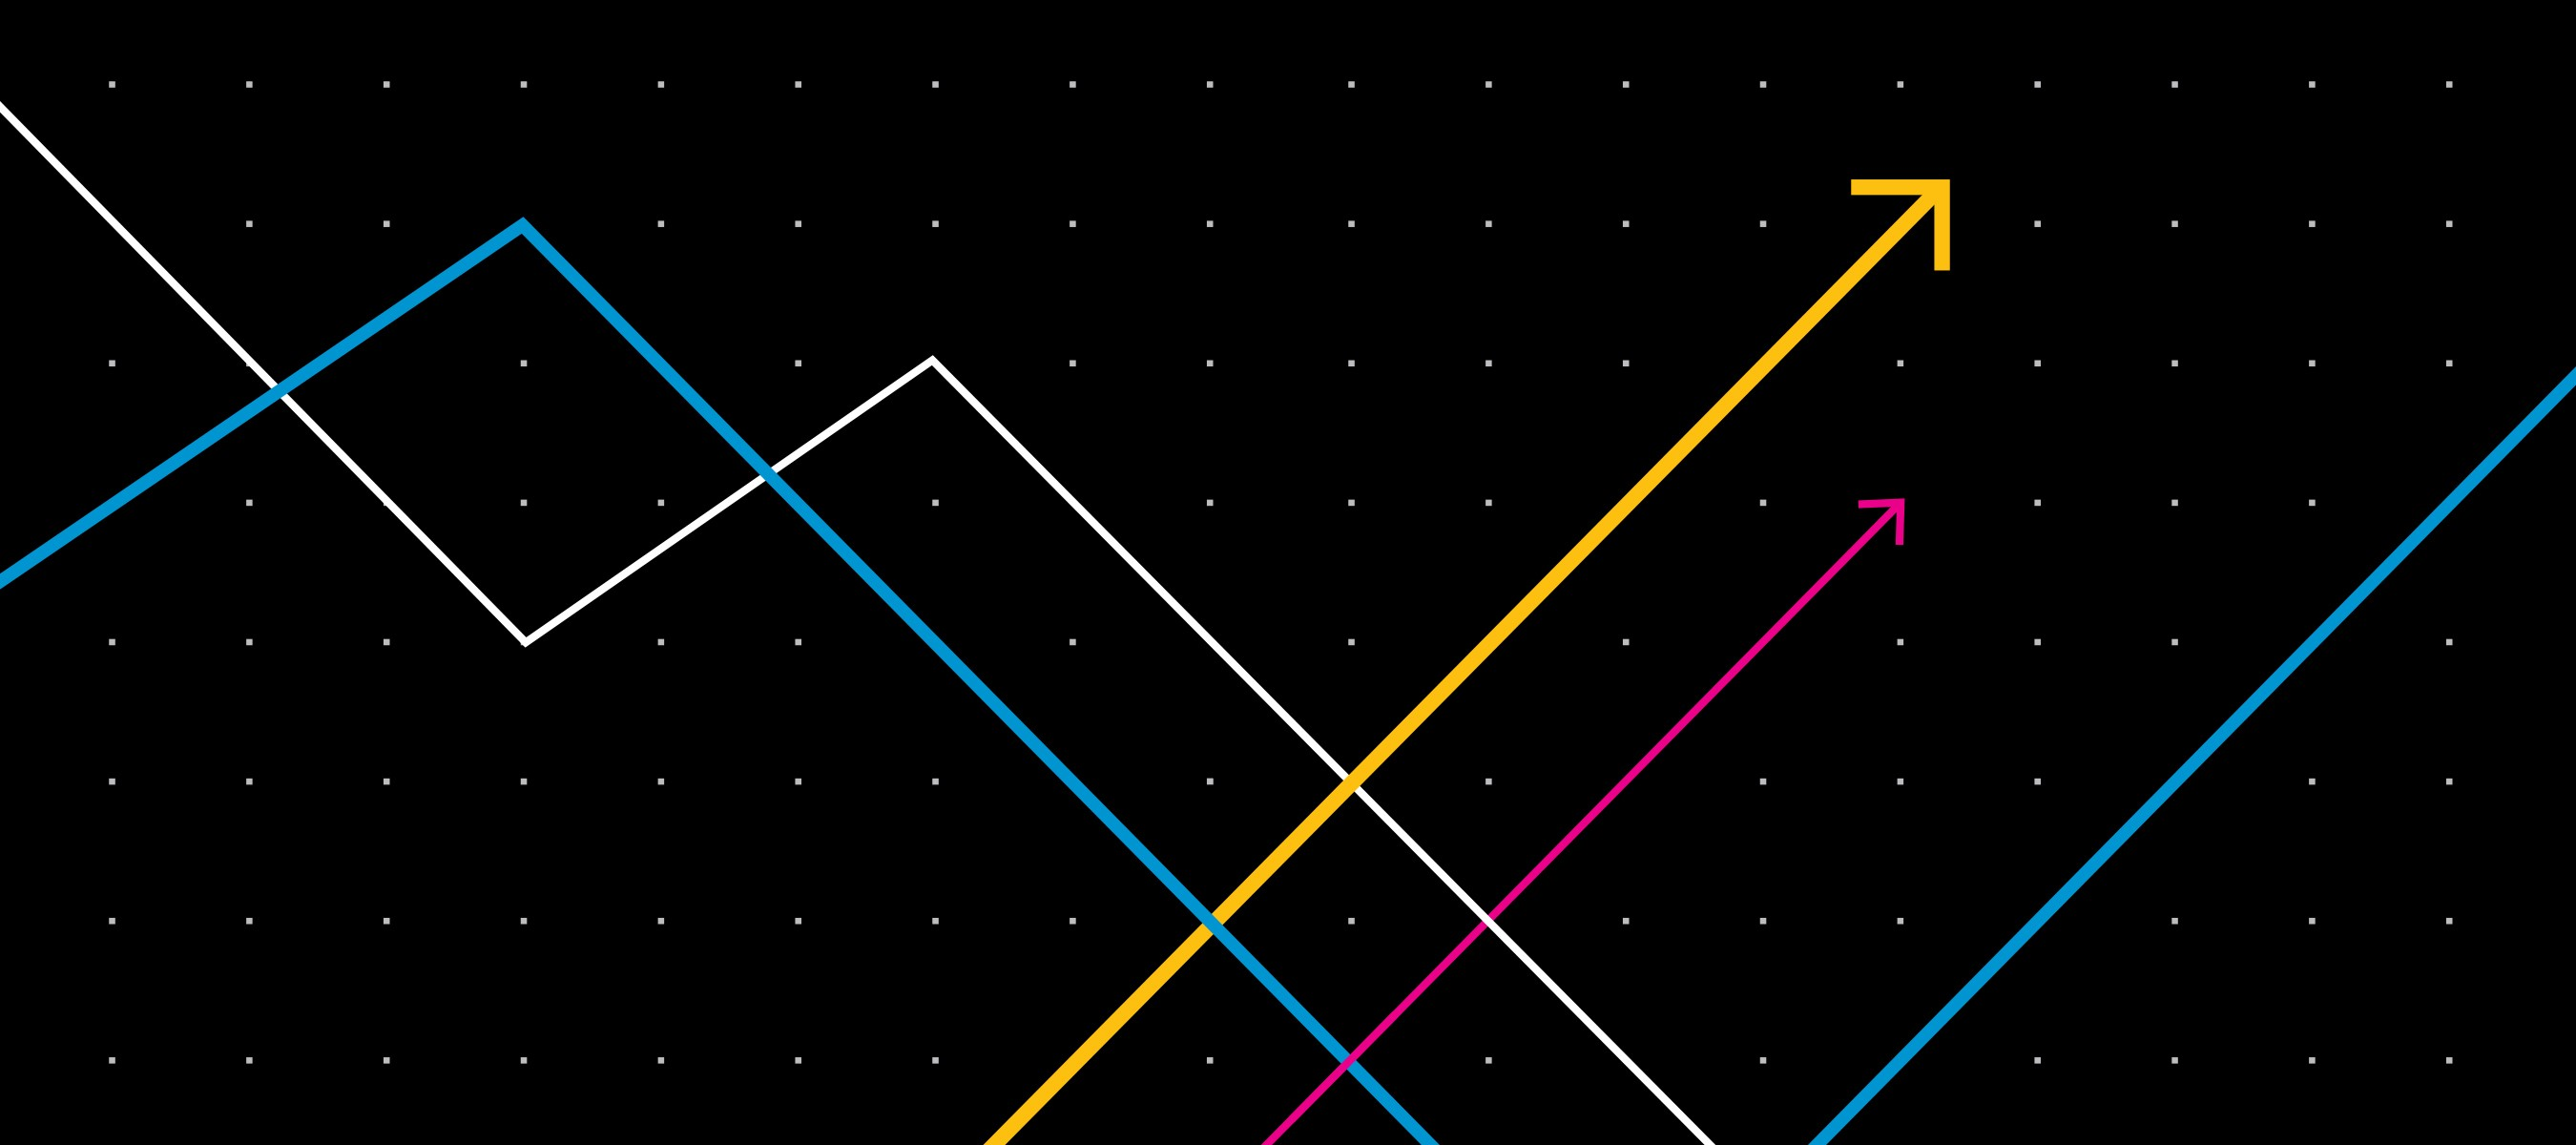
\includegraphics{images/cover.jpg}}
    
    \vspace{0.35in}
    \noindent\textcolor{urban-blue}{\MakeUppercase{\textbf{Research Report}}}
    
    \titlereport{Opt-In Statistical Disclosure Protections}
    
    \vspace{-0.25in}
    
    \reportsubtitle{Empowering Survey Respondents to Improve Data Quality}
    % Multiple column author names - change the "4" to the number of desired columns
    \begin{multicols}{2}
        \authorfont{Aaron R. Williams}
        
        \authorfont{Jennifer Andre}
      
    \end{multicols}
    
    \datefont{August 2023}

    % Add logo
    \begin{textblock*}{4.5in}[1, 1](5.5in, 10.5in)
        \noindent
\includegraphics[width=4.5in]{images/cover-footer.jpg}
    \end{textblock*}
\end{titlepage}

%%%%%%%%%%%%%%%%%%%%%%%%%%%%%%%%%%%% About Urban %%%%%%%%%%%%%%%%%%%%%%%%%%%%%%%%%%%
\thispagestyle{empty} % Removed Page Number
\begin{figure}
    
\includegraphics[width=1.5in]{images/logo.png}
\end{figure}
\vspace*{-0.5in}
\about{About the Urban Institute}\\
\vspace{-5pt}
\boilerplate{The nonprofit Urban Institute is a leading research organization dedicated to developing evidence-based insights that improve people’s lives and strengthen communities. For 50 years, Urban has been the trusted source for rigorous analysis of complex social and economic issues; strategic advice to policymakers, philanthropists, and practitioners; and new, promising ideas that expand opportunities for all. Our work inspires effective decisions that advance fairness and enhance the well-being of people and places.}

\vspace*{\fill}
\begin{singlespace}
    \noindent Copyright ©\tbf{Month Year}. Urban Institute. Permission is granted for reproduction of this file, with attribution to the Urban Institute. Cover image by \tbf{Tim Meko}.
\end{singlespace}

\cleardoublepage

\setcounter{page}{3}
\begin{singlespace}
    \tableofcontents
\end{singlespace}

\thispagestyle{empty}

% Footer Formatting: DO NOT CHANGE -----------------------------------
\fancyfoot{}

\fancyfoot[LE]{\colorbox{urban-footergray}{\makebox(0.2, 0.12)[r]{\fontsize{7.5}{0}\selectfont\bfseries{\MakeUppercase{}\hspace{0.2in}}}}\colorbox{urban-gold}{\makebox(0.2, 0.12)[c]{\fontsize{7.5}{0}\selectfont\bfseries{\MakeUppercase\thepage}}}\colorbox{urban-footergray}{\makebox(5.64, 0.12)[r]{\fontsize{7.5}{0}\selectfont\bfseries{\MakeUppercase{Acknowledgments}\hspace{0.2in}}}}}

\fancyfoot[RO]{\colorbox{urban-footergray}{\makebox(5.64, 0.12)[l]{\fontsize{7.5}{0}\selectfont\bfseries{\hspace{0.2in}\MakeUppercase{Acknowledgments}}}}\colorbox{urban-gold}{\makebox(0.2, 0.12)[c]{\fontsize{7.5}{0}\selectfont\bfseries{\MakeUppercase\thepage}}}\colorbox{urban-footergray}{\makebox(0.2, 0.12)[r]{\fontsize{7.5}{0}\selectfont\bfseries{\MakeUppercase{}\hspace{0.2in}}}}}
% Footer Formatting: DO NOT CHANGE -----------------------------------
%%%%%%%%%%%%%%%%%%%%%%%%%%%%%%%%%%%% Acknowledgments %%%%%%%%%%%%%%%%%%%%%%%%%%%%%%%%%%%%
\part{Acknowledgments}

This report was funded by \tbf{[insert your funder name(s) here].} We are grateful to them and to all our funders, who make it possible for Urban to advance its mission. 

The views expressed are those of the \tbf{author/authors} and should not be attributed to the Urban Institute, its trustees, or its funders. Funders do not determine research findings or the insights and recommendations of Urban experts. Further information on the Urban Institute’s funding principles is available at \textcolor{urban-url}{urban.org/fundingprinciples}.

\tbf{[Add any other thanks and contract details here. It may be appropriate to also acknowledge your funder’s funder(s). When in doubt, please check with your center director and Contracts.]}

% Footer Formatting: DO NOT CHANGE -----------------------------------
\fancyfoot{}

\fancyfoot[LE]{\colorbox{urban-footergray}{\makebox(0.2, 0.12)[r]{\fontsize{7.5}{0}\selectfont\bfseries{\MakeUppercase{}\hspace{0.2in}}}}\colorbox{urban-gold}{\makebox(0.2, 0.12)[c]{\fontsize{7.5}{0}\selectfont\bfseries{\MakeUppercase\thepage}}}\colorbox{urban-footergray}{\makebox(5.64, 0.12)[r]{\fontsize{7.5}{0}\selectfont\bfseries{\MakeUppercase{Executive Summary}\hspace{0.2in}}}}}

\fancyfoot[RO]{\colorbox{urban-footergray}{\makebox(5.64, 0.12)[l]{\fontsize{7.5}{0}\selectfont\bfseries{\hspace{0.2in}\MakeUppercase{Executive Summary}}}}\colorbox{urban-gold}{\makebox(0.2, 0.12)[c]{\fontsize{7.5}{0}\selectfont\bfseries{\MakeUppercase\thepage}}}\colorbox{urban-footergray}{\makebox(0.2, 0.12)[r]{\fontsize{7.5}{0}\selectfont\bfseries{\MakeUppercase{}\hspace{0.2in}}}}}
% Footer Formatting: DO NOT CHANGE -----------------------------------
%%%%%%%%%%%%%%%%%%%%%%%%%%%%%%%%%%%% Executive %%%%%%%%%%%%%%%%%%%%%%%%%%%%%%%%%%%%%%%%%
\part{Executive Summary}

\intropara{Body Text style or Chapter Intro Para style here (text shown is in Chapter Intro Para). If you do not have an executive summary, remove this section.}

\section{First-Level Heading in Title Case (Heading 2 style)}

Body Text style for first paragraph under a heading.

Body Text First Indent style for all subsequent paragraphs. \tbf{To add an endnote, use the Insert Endnote function. Endnotes will automatically appear in the Notes section after the appendixes.}\endnote{Endnotes should appear automatically under the Notes heading. If they’re showing up somewhere else, ask your editor or your center’s Word expert for assistance.}

\subsection{Second-Level Heading in Title Case (Heading 3 style)}

Body Text style for first paragraph under a heading.

Body Text First Indent style for all subsequent paragraphs.


\subsubsection{Third-level heading; all caps is built into style (heading 4 style)}

Body Text style for first paragraph under a heading.

Body Text First Indent style for all subsequent paragraphs.

\part{Opt-In Statistical Disclosure Protections}

\section{Introduction}

People generate and share data about themselves every day when they
browse the web, interact with government services, and respond to
questionnaires, and they should be empowered to make decisions about how
these data are accessed and used. Currently, disclosure protection
policies at the US Census Bureau do not allow for such empowerment --
respondents to questionnaires like the decennial census and the American
Community Survey are all subjected to disclosure protections. Data for
all respondents are, by default, masked with some form of statistical
disclosure control, and those who may wish to see themselves accurately
reflected in the data are unable to do so. Statistical disclosure
control may inflict greater damage to the accuracy of information for
certain groups, such as smaller race and ethnicity groups, relative to
others.

In this brief, we explore a new framework for disclosure protections
that would require respondents to actively opt in to disclosure
protections. Responses for those who opt in would be treated with
disclosure protections, while responses for those who forego protections
would remain unchanged in statistical product outputs. We present two
demonstration studies, the first using an opt-in local differential
privacy approach for the decennial census, and the second using an
opt-in synthetic data approach for the American Community Survey. In
both cases, we seek to explore the impact of varying the rate of opting
in to disclosure protections on data quality and the associated privacy
consequences. We especially examine the impact for small racial/ethnic
groups, including the impact on quality and privacy if some groups opt
in at higher rates than others.

We aim to test the feasibility of this potential solution path,
contributing to ongoing public discussions and debate about disclosure
protections and public data quality involving researchers, public data
users, and other stakeholders. This solution would have wide-ranging
implications, including operational changes, new outreach strategies,
and many complex legal questions about Title 13 and other regulations.
The findings we present here provide early evidence on the impact of
turning privacy disclosure choices over to participants.

\section{Background}

The primary goal of this report is to present the opt in privacy
framework and early evidence on the impact of such a framework on two
demonstrations. The data privacy literature is extensive, and we assume
a baseline knowledge of certain key concepts. In this section, we
provide a brief overview of a few key concepts, as well as a review of
disclosure avoidance at the US Census Bureau.

\subsection{Data Privacy Key Terms}

\emph{Statistical Disclosure Control Methods}

Statistical Disclosure Control (SDC) methods are used to release
sensitive or confidential data products while preserving the
confidentiality of the data. Traditional SDC methods include
suppression, rounding, top- and bottom-coding, and synthetic data
generation.

\emph{Differential Privacy}

Differential Privacy (DP) is a formal definition of privacy, meaning
that DP methods meet certain mathematical properties and guarantees.
With DP, it is possible to quantify the worst-case disclosure risk of a
data release using a ``privacy-loss budget.'' The privacy-loss budget is
qunatified with parameters like \(\epsilon\) and \(\delta\).

\emph{Utility-Privacy Trade-off}

When applying disclosure avoidance methods to confidential data, there
exists a central tension between the usefulness or quality of the
resulting ``noisy'' data and the amount of privacy risk. Before any
noise infusion, confidential data have the highest possible utility, but
also have high privacy risks. Efforts to improve disclosure protections
via SDC methods can reduce these privacy risks, but also may worsen
overall data quality and usefulness for intended analyses or other
applications. With DP methods, it is possible to ``tune'' the balance
between utility and privacy by changing the value of \(\epsilon\), with
lower values of \(\epsilon\) corresponding to greater noise infusion,
implying lower data quality and higher disclosure protection. With
methods that are not formally private, the utility-privacy trade-off is
ad hoc.

\subsection{The US Census Bureau and Disclosure Avoidance}

The US Census Bureau is tasked with providing high quality data about
the US and its people. These data are of enormous consequence for the
public, serving as the basis for political representation, community
funding and planning, and key research. Given these use cases, the
accuracy and quality of Census Bureau products is crucial.

Decennial census statistical products are used for congressional
apportionment, redistricting, federal funding allocations, planning and
decision-making for government and business organizations, and informing
many other surveys (Mather and Scommegna 2019). The American Community
Survey (ACS) is used to inform federal policymaking and program
delivery, state and local service provision (e.g., roads and schools),
and research and analysis by nongovernmental organizations (United
States Census Bureau 2017). In fiscal year 2015, 132 federal programs
used Census Bureau data to allocate more than \$675 billion in funds to
state and local communities (Hotchkiss and Phelan 2017). Decennial
census and ACS data are also foundational to racial equity analytics,
enabling researchers to answer important research and policy questions
(Axelrod, Ramos, and Bullied 2022).

In addition to conducting surveys and releasing high quality public
data, the Census Bureau is also obligated to protect the confidentiality
of individual respondents reflected in these data products. The Census
Bureau's approach to safeguarding the identities of respondents in
publicly released data is informed by its interpretation of Section 9 of
Title 13 of the US Code, enacted in 1954. This approach has evolved over
the years, especially in response to advances in computing technologies
and attack methods (Hotz and Salvo 2022). In 2018, the Census Bureau
announced its intention to ``modernize how we protect respondent
confidentiality,'' including the adoption of Differential Privacy (DP)
(J. M. Abowd 2018). This move was motivated by certain benefits of DP
over traditional disclosure limitation, including more robust
protections and greater transparency (J. Abowd et al. 2022).

For the 2020 Decennial Census, the Census Bureau updated their
Disclosure Avoidance System (DAS) from traditional swapping algorithms
to the TopDown Algorithm (TDA), which refers to a system of DP
mechanisms for privacy loss accounting, along with optimization
algorithms and post-processing. The TDA satisfies zero-concentrated DP
(\(\rho\)-zCDP), a relaxation of pure DP. As a formally private method,
the privacy protections can be quantified, and the Census Bureau does
translate the \(\rho\)-zCDP privacy parameter \(\rho\) to the
corresponding values of \(\epsilon\) and \(\delta\) (Bowen, Williams,
and Pickens 2022; J. Abowd et al. 2022).

In contrast, the Census Bureau has conceded that the ``science does not
yet exist to comprehensively implement a formally private solution for
the ACS'' (Daily 2022). Instead, they are currently exploring the
feasibility of a fully synthetic public-use microdata file and
accompanying validation server. In both cases, all respondents are
subjected to disclosure protections, even those who might otherwise
prefer to see their data accurately reflected.

\section{Opt-In Privacy Framework and Implications}

In our demonstrations, we imagine a framework for disclosure protection
in which respondents would be asked to actively opt into statistical
disclosure control methods. Those who do not opt-in would simply
contribute their true data to statistical products. The choices we make
to build this framework may have significant ethical and legal
implications, discussed in this section.

\subsection{Opt In Framework Ethical Implications}

The adoption of a framework requiring respondents to opt in to
disclosure protections has various ethical considerations. First, a
major challenge upon implementation of such a framework would be a
significant knowledge gap for respondents. The Census Bureau or any
other organization would need to carry out extensive outreach efforts
and design plain-language explanations to ensure that respondents
understand what they are or are not opting into. It is crucial for
respondents to understand the implications of their opt-in choice not
only for the privacy of their personal information, but also for the
resulting data quality and the downstream impact on their community.

Second, there are ethical considerations in the framing of the opt-in
decision and the administration of the question in a survey. For this
project, we intentionally chose language of ``opting in'' to disclosure
avoidance protections, treating the decision to forego protections as
the default and requiring an additional step for those desiring
additional protections. This is in contrast to language of ``opting
out'', which would treat disclosure avoidance protections as the default
position. Additionally, we made the simplifying assumption that the
primary survey respondent, or householder, makes the opt in decision for
all members of the household. This choice may be appropriate if the
householder is the parent or legal guardian of a minor in the household,
but may not be appropriate for other adults in the household who may
disagree with the respondent's opt-in decision.

Finally, any application of an opt in framework to disclosure avoidance
methods must consider the impact of one respondent choosing to forego
protections of the privacy risks of respondents who do opt in. The
mathematical guarantees of differential privacy allow for individuals to
forego protections without decreasing other respondents' protection, but
this is not guaranteed in non-formally private methods like synthetic
data generation.

\subsection{Opt In Framework Legal Implications}

In addition to ethical considerations, the implementation of an opt in
disclosure avoidance framework would also have significant legal
implications. Most notably, the implementation of this type of framework
would most likely require a change to Title 13 of the US Code, which
could trigger complex legal arguments and potential politicization.

\section{Demonstration 1: Local Differential Privacy for the Decennial Census}

The Census Bureau deployment of DP for the 2020 Decennial Census uses a
global approach in which tabulated cells of confidential responses in a
series of data tables are infused with noise by a central curator (the
Census Bureau). All census respondents are automatically subjected to
the DAS, even those who might otherwise wish to see their data reflected
accurately, without any noise. Further, the noise that is injected into
tabulated data cells is independent of the size of the population in the
cell. In effect, there is more relative error added for small groups
than for larger ones. This could lead to worse data quality for small
groups such as some racial/ethnic groups and, as a result of inaccurate
representation in the data, these groups could receive inadequate
funding and incorrect research findings.

\subsection{Local Differential Privacy}

To allow for individual-level opt-in, we move from a central DP
approach, in which the Census Bureau as a data curator would add noise
to all respondents, to a local DP approach, allowing for some
respondents to opt in and others to forego disclosure protections.
Typically, a local model assumes that a central curator cannot be
trusted, and so a respondent adds noise to their data before sending it
to the curator. For this use case, we can imagine a slight variation on
this approach in which the trusted Census Bureau still receives all data
in its confidential form, and then infuses noise only for respondents
who opt in.

Many local DP mechanisms are based on the concept of Randomized
Response, first proposed by Warner (1965). The central idea is that a
survey respondent flips a coin, and the result of the coin flips
determines if they answer a yes/no question with the true answer or not.
The randomization of the coin flip infuses the noise that grants
disclosure protections (Near and Abuah 2022).

We use Generalized Random Response (GRR) for our use case, allowing us
to move from a binary coin flip to a setting with higher cardinality.
With GRR, we turn the entire domain of potential responses into a
histogram and randomly switch observations based on a rate determined by
the privacy loss budget, \(\epsilon\). We then tabulate a resulting
histogram of counts and apply an adjustment to account for the randomly
perturbed responses (Wang et al. 2020).

\subsection{Data}

For this demonstration, we use person-level records from the 2010
Decennial Census Stateside Public Use Microdata Sample. This sample
contains records representing 10 percent of housing units, and the
people residing in them, along with 10 percent of people living in group
quarters. We restrict our sample to Washington, DC and Iowa because the
former has two large racial/ethnic groups, while the latter is more
homogeneous. These data contain demographic and household
characteristics about respondents, including age, race, ethnicity, and
sex.

\subsection{Simulations}

For our simulation approach, we run iterations of a disclosure mechanism
to generate noisy histograms of counts for a set of defined attributes.
We focus on two disclosure mechanisms to compare a standard global
approach to a local opt-in approach. The first is a Laplace sanitizer, a
global method in which cells are infused with noise from a Laplace
distribution. The Laplace distribution is centered at zero and the
variability is the ratio of the privacy loss budget, \(\epsilon\), over
the \(l_1\)-global sensitivity of the statistic (Dwork et al. 2006;
Williams and Bowen 2023). The second is the previously described GRR
method, a local method in which individuals who opt in to disclosure
protections report a true response with probability
\(p = \frac{e^\epsilon}{e^\epsilon + d - 1}\), where \(d\) is the
overall cardinality of possible response values. Otherwise, the record
is randomly replaced with another combination of fields. Though the TDA
deployed by the Census Bureau is a more complicated series of algorithms
and processing steps than the simple Laplace mechanism presented here,
this simplification allows us to compare more easily with a simple local
approach and focus specifically on the impact of the opt in framework on
data quality.

The specifications for our simulations are as follows. For each
combination of specifications, we run 100 iterations of each disclosure
mechanism.

\begin{itemize}
\tightlist
\item
  Scenarios: the set of grouping attributes for the resulting histogram
  frequencies

  \begin{itemize}
  \tightlist
  \item
    Scenario 1 (cardinality = 2)

    \begin{itemize}
    \tightlist
    \item
      Hispanicity: Hispanic or Latino, Not Hispanic or Latino
    \end{itemize}
  \item
    Scenario 2 (cardinality = 24)

    \begin{itemize}
    \item
      Age bucket: Child (0-17), Adult (18-64), Senior (65+)
    \item
      Race/Ethnicity: White alone, Black or African American alone,
      Other alone, or Hispanic or Latino (any race)
    \item
      Sex: Male, Female
    \end{itemize}
  \end{itemize}
\item
  Privacy loss budget, \(\epsilon\)

  \begin{itemize}
  \tightlist
  \item
    1
  \item
    5
  \item
    10
  \item
    20
  \end{itemize}
\item
  Opt-in rate: the probability that respondents opt in to disclosure
  protections

  \begin{itemize}
  \item
    0.01
  \item
    0.1
  \item
    0.5
  \item
    0.9
  \item
    1
  \end{itemize}
\end{itemize}

\subsection{Evaluation}

We evaluate the results of these simulations using bias and accuracy
metrics, comparing the noisy histograms generated under each privacy
approach to each other and to the true values. We use mean percent error
to evaluate bias, or the tendency for noisy estimates to systematically
move in one direction relative to the true values. We use absolute mean
percent error to evaluate accuracy, or the closeness of noisy estimates
to the true values.

\subsection{Results and Discussion}

\textbf{Local DP Methods Result in Overall Lower Accuracy than Global
Methods}

For Scenario 1, we focus primarily on results allowing us to compare the
performance of the local GRR method to the central Laplace method. With
a cardinality of just 2 (Hispanic or Latino, Not Hispanic or Latino),
this scenario allows for the most similar comparison with the global
method (in which epsilon is allocated to just one statistic).

Figure \ref{fig:methods-bias} shows the distribution of bias metrics
from our simulations at the defined levels of \(\epsilon\) and opt in
rate. Both the local and central methods are unbiased, with the
distribution of mean percent error values centered around zero.

\begin{figure}[!htb]
    \centering
    \caption{Local and Central DP Approaches are Similarly Unbiased}
    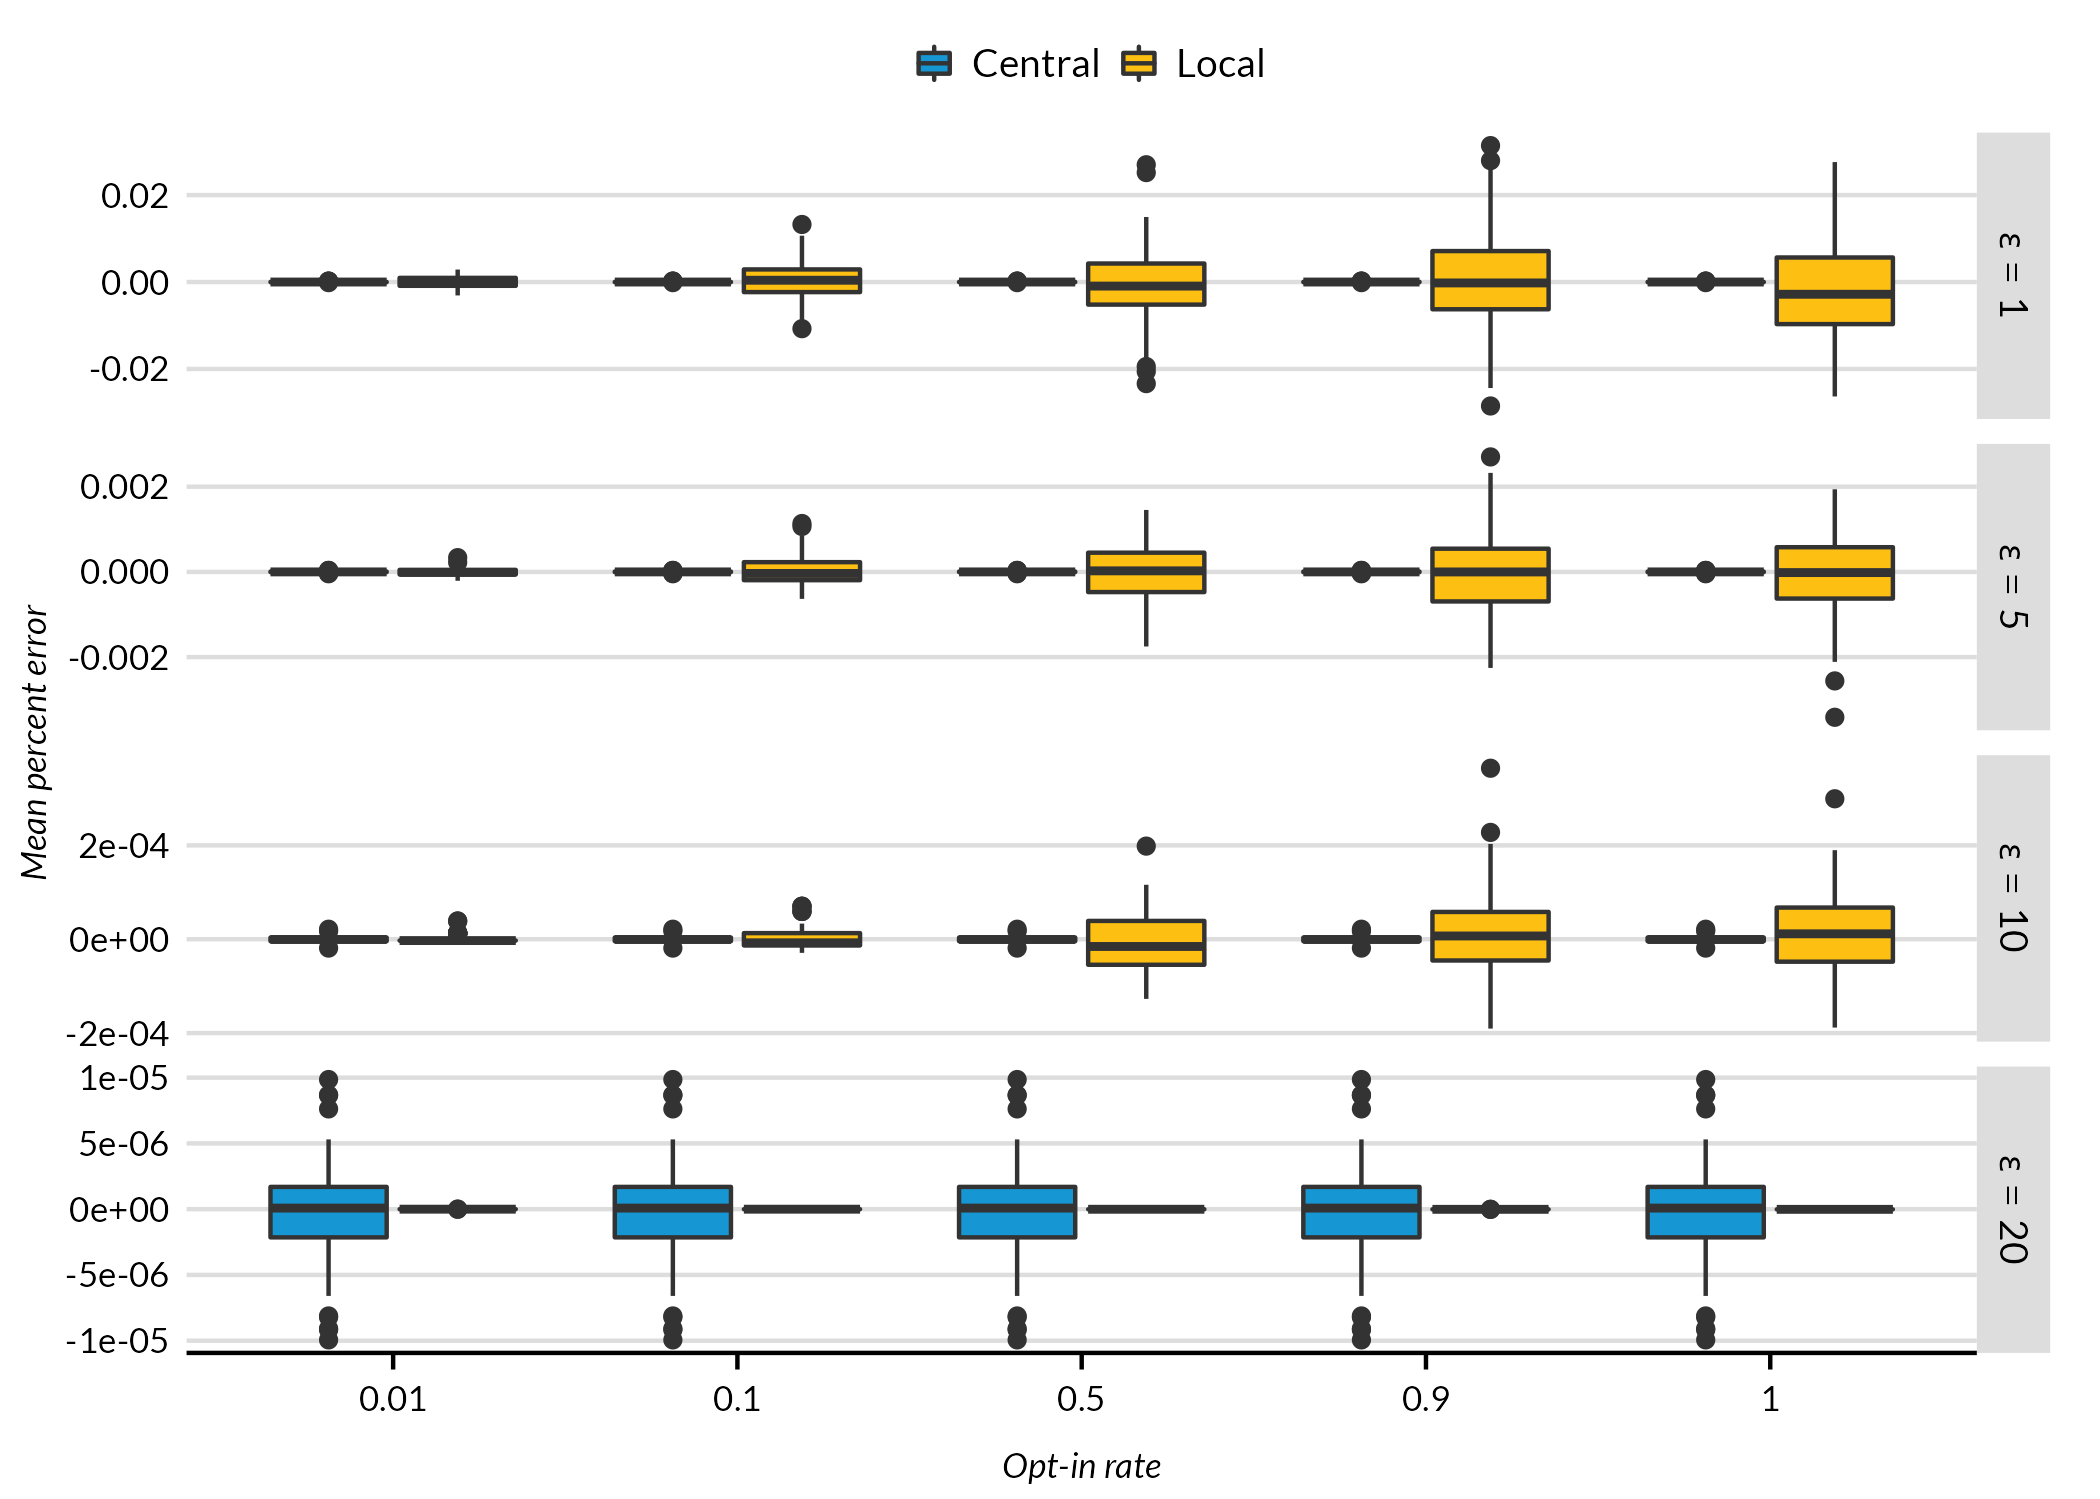
\includegraphics[width=4in]{../figures/methods_bias.png}
    \label{fig:methods-bias}
\end{figure}

Figure \ref{fig:methods-accuracy} shows the distribution of accuracy
metrics from our simulations at the defined levels of epsilon and opt in
rate.

\begin{figure}[!htb]
    \centering
    \caption{Local Method Outperforms Central Method Only with Very High Privacy Loss Budget}
    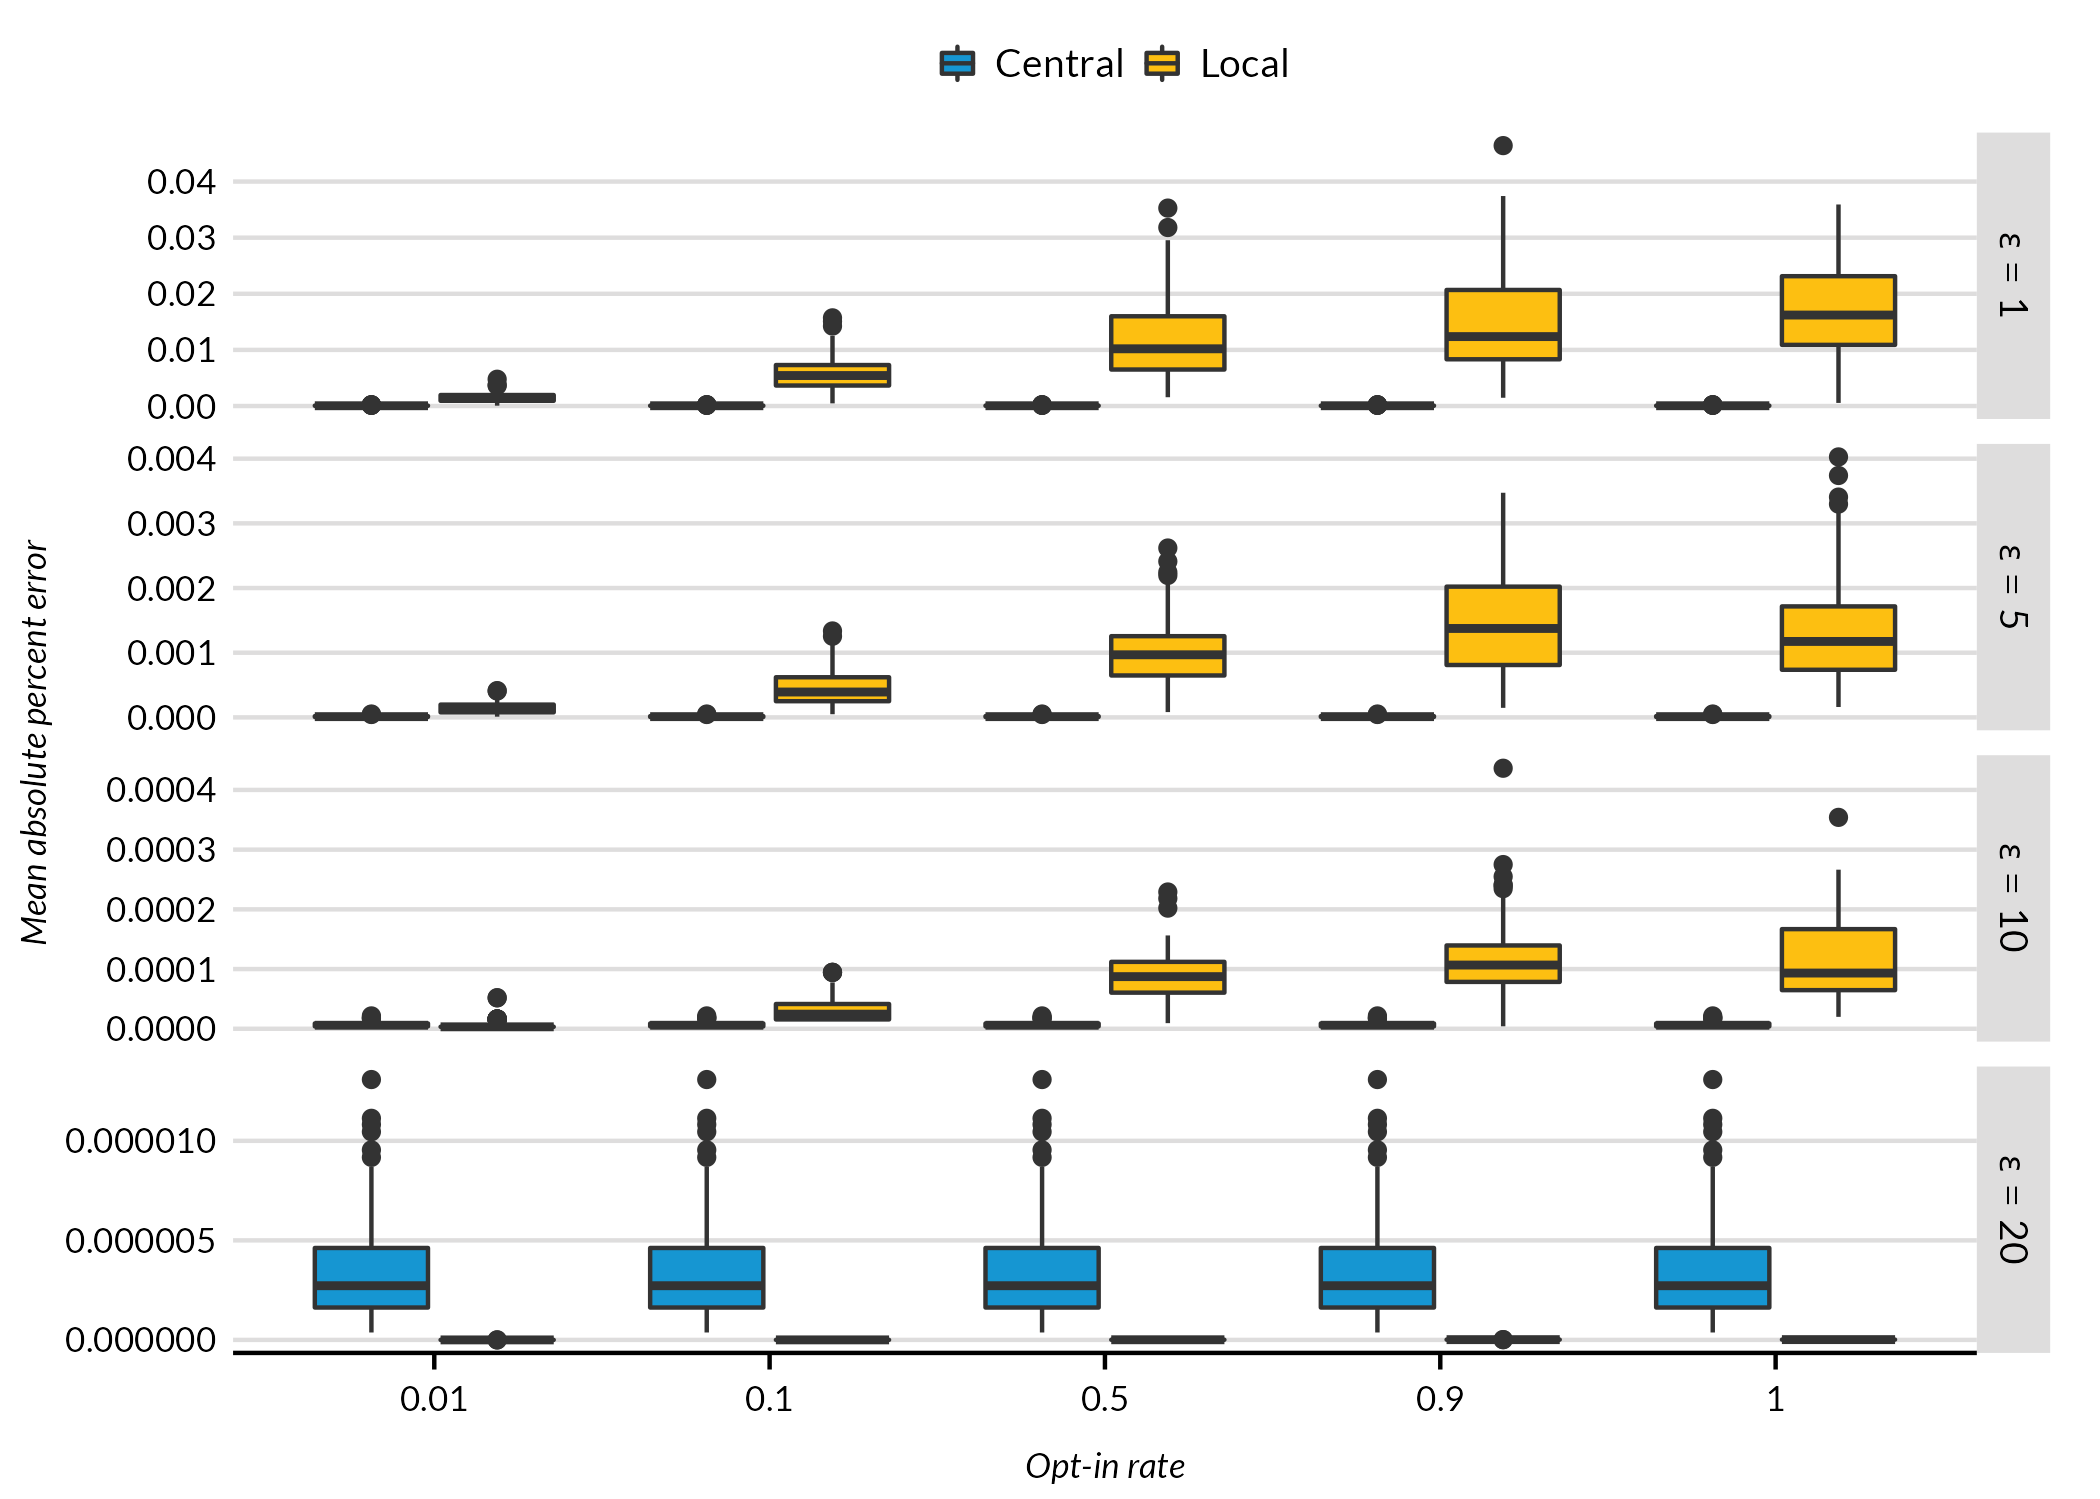
\includegraphics[width=4in]{../figures/methods_accuracy.png}
    \label{fig:methods-accuracy}
\end{figure}

Figure \ref{fig:methods-accuracy} demonstrates two key takeaways about
the accuracy of these methods. First, the opt-in framework approach does
improve the overall accuracy of the local GRR method. As we decrease the
level of opt in, the width of the mean percent error distribution
shrinks and moves closer to zero. However, the second key takeaway is
that the central method significantly outperforms the local method in
terms of accuracy at nearly every tested level of \(\epsilon\) and opt
in rate, even with very small opt in rates. The local method only
outperforms the central method with a very high privacy loss budget of
\(\epsilon\) = 20, and the errors for both methods are very small for
that level of privacy loss anyway.

While the opt-in local approach does improve the accuracy of estimates
with lower levels of opt in, this improvement alone is unfortunately not
enough to justify a switch from a central model to a local model.
Existing local DP methods cannot offer the same level of accuracy as
central methods, especially for datasets with even higher cardinality.
However, the potential to improve data quality results with a local
method and opt-in framework motivates greater focus on developing local
DP methods in the future.

\textbf{Opt-in Privacy Offers the Potential to Improve Data Quality for
Small Groups}

Although existing local DP methods may be disappointing for overall
accuracy, an opt-in local DP framework still offers the potential to
improve data quality for small groups. Data quality may be especially
improved for groups that opt-in at relatively lower rates than others.
For Scenario 2, we focus on results allowing us to compare differences
in data quality by racial/ethnic group.

Figures \ref{fig:groups_dc} and \ref{fig:groups_ia} show the
distribution of accuracy results for the specified opt in rates for each
racial/ethnic group (using \(\epsilon\) = 1), separately by state.

\begin{figure}[!htb]
    \centering
    \caption{Accuracy By Racial/Ethnic Group, Washington, DC}
    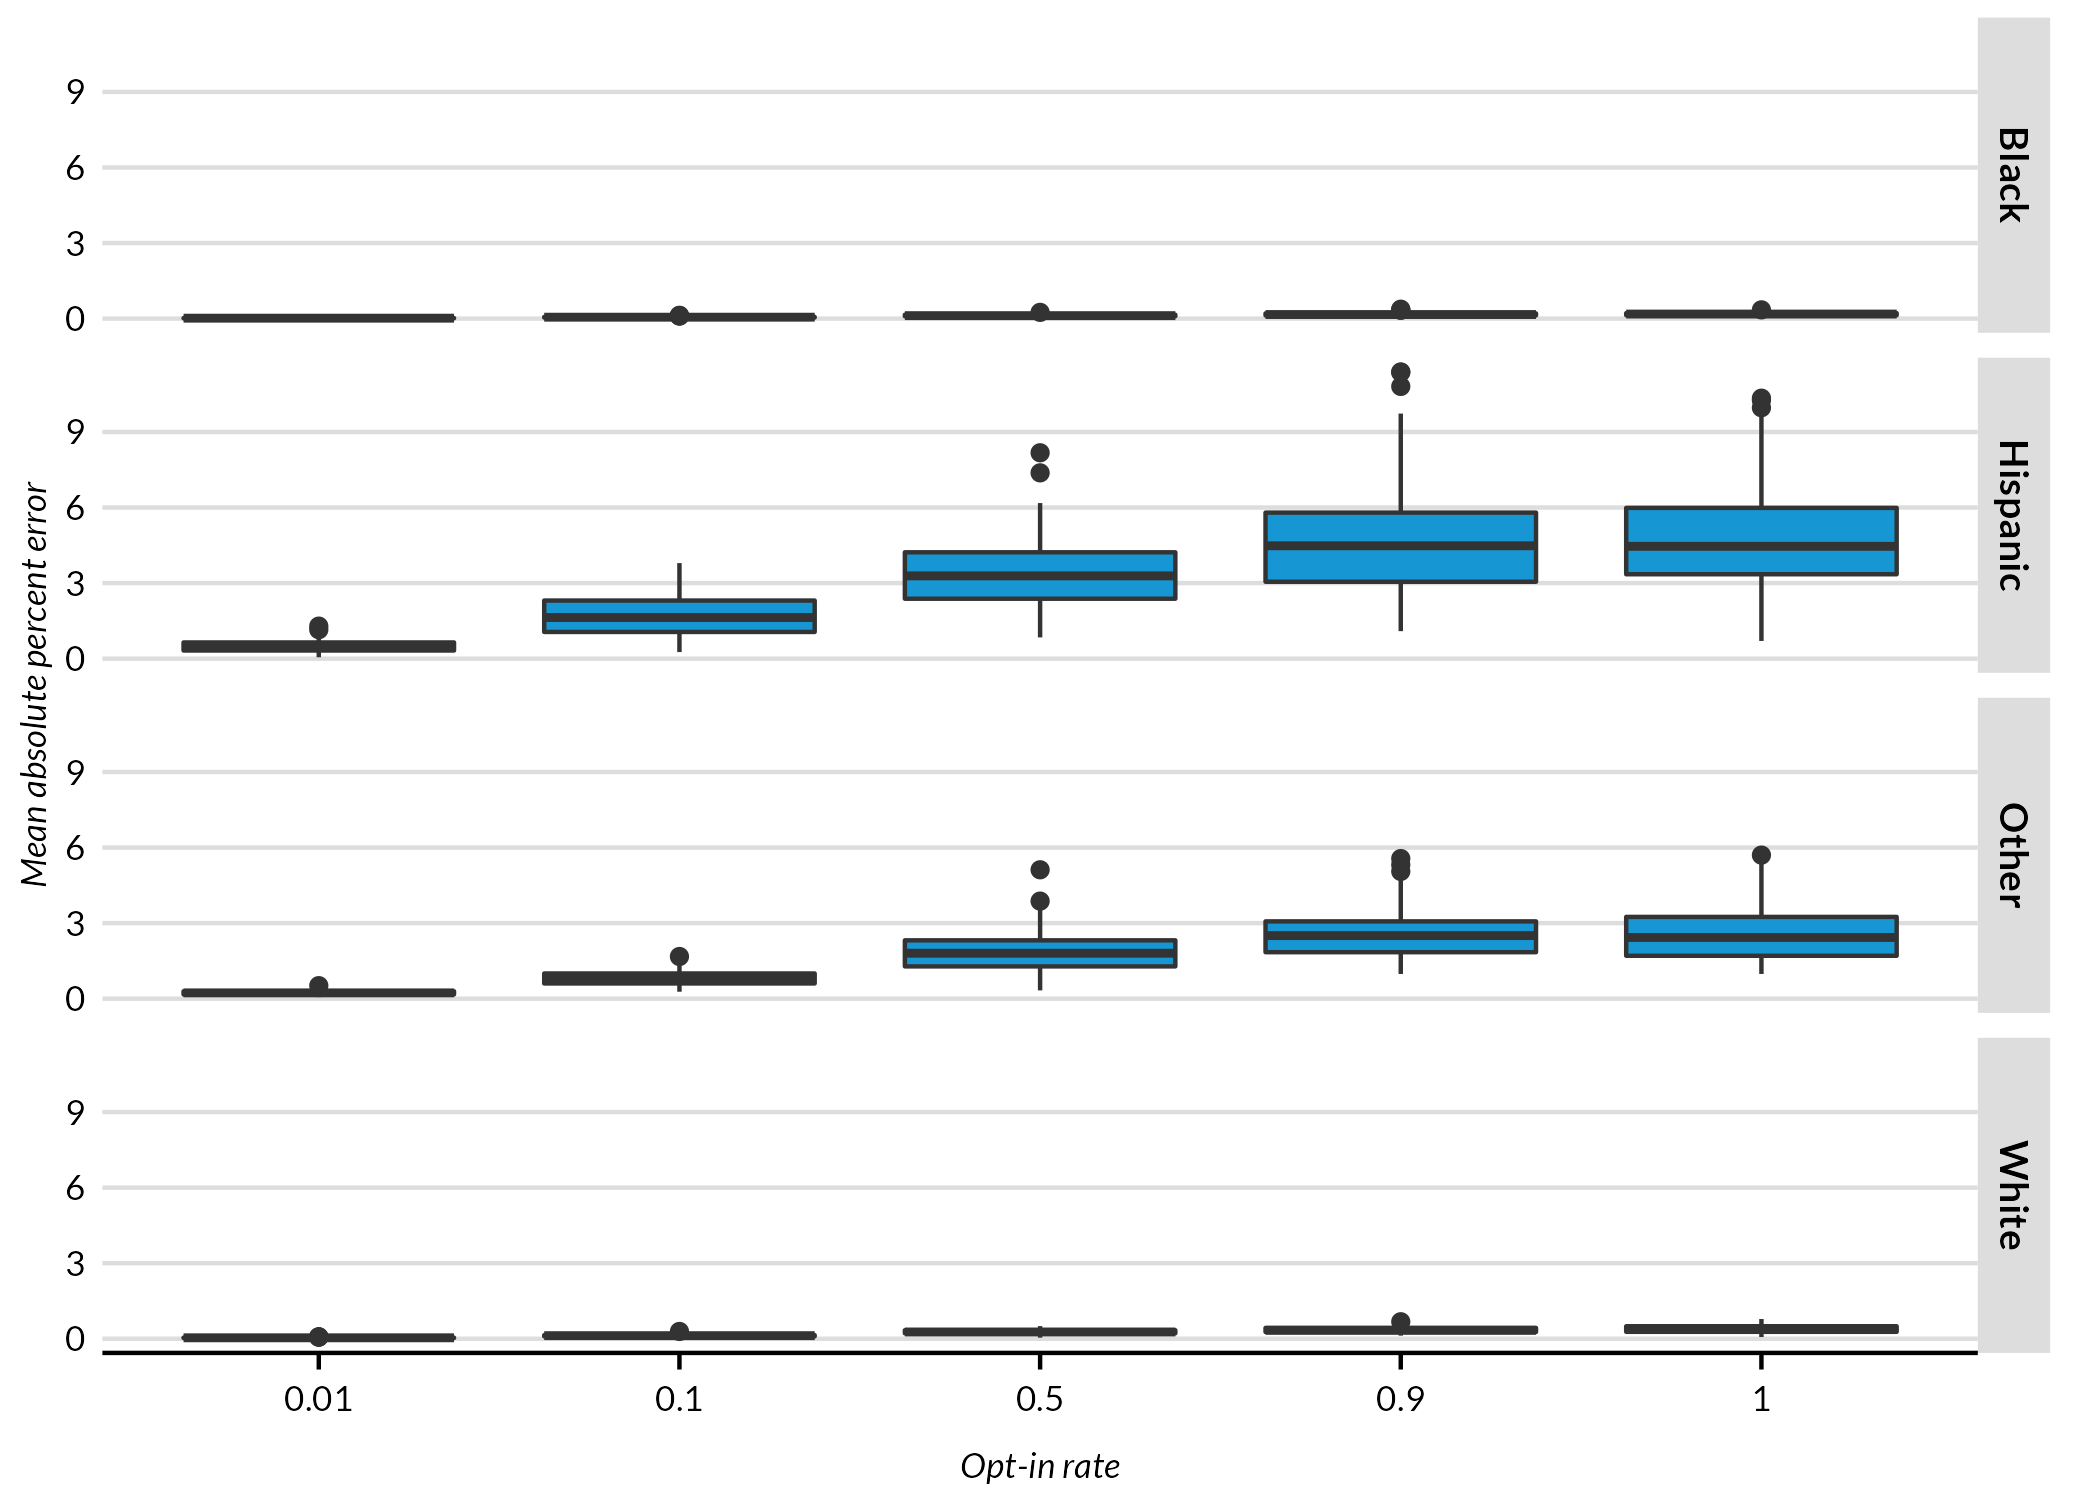
\includegraphics[width=4in]{../figures/groups_dc.png}
    \label{fig:groups_dc}
\end{figure}

\begin{figure}[!htb]
    \centering
    \caption{Accuracy By Racial/Ethnic Group, Iowa}
    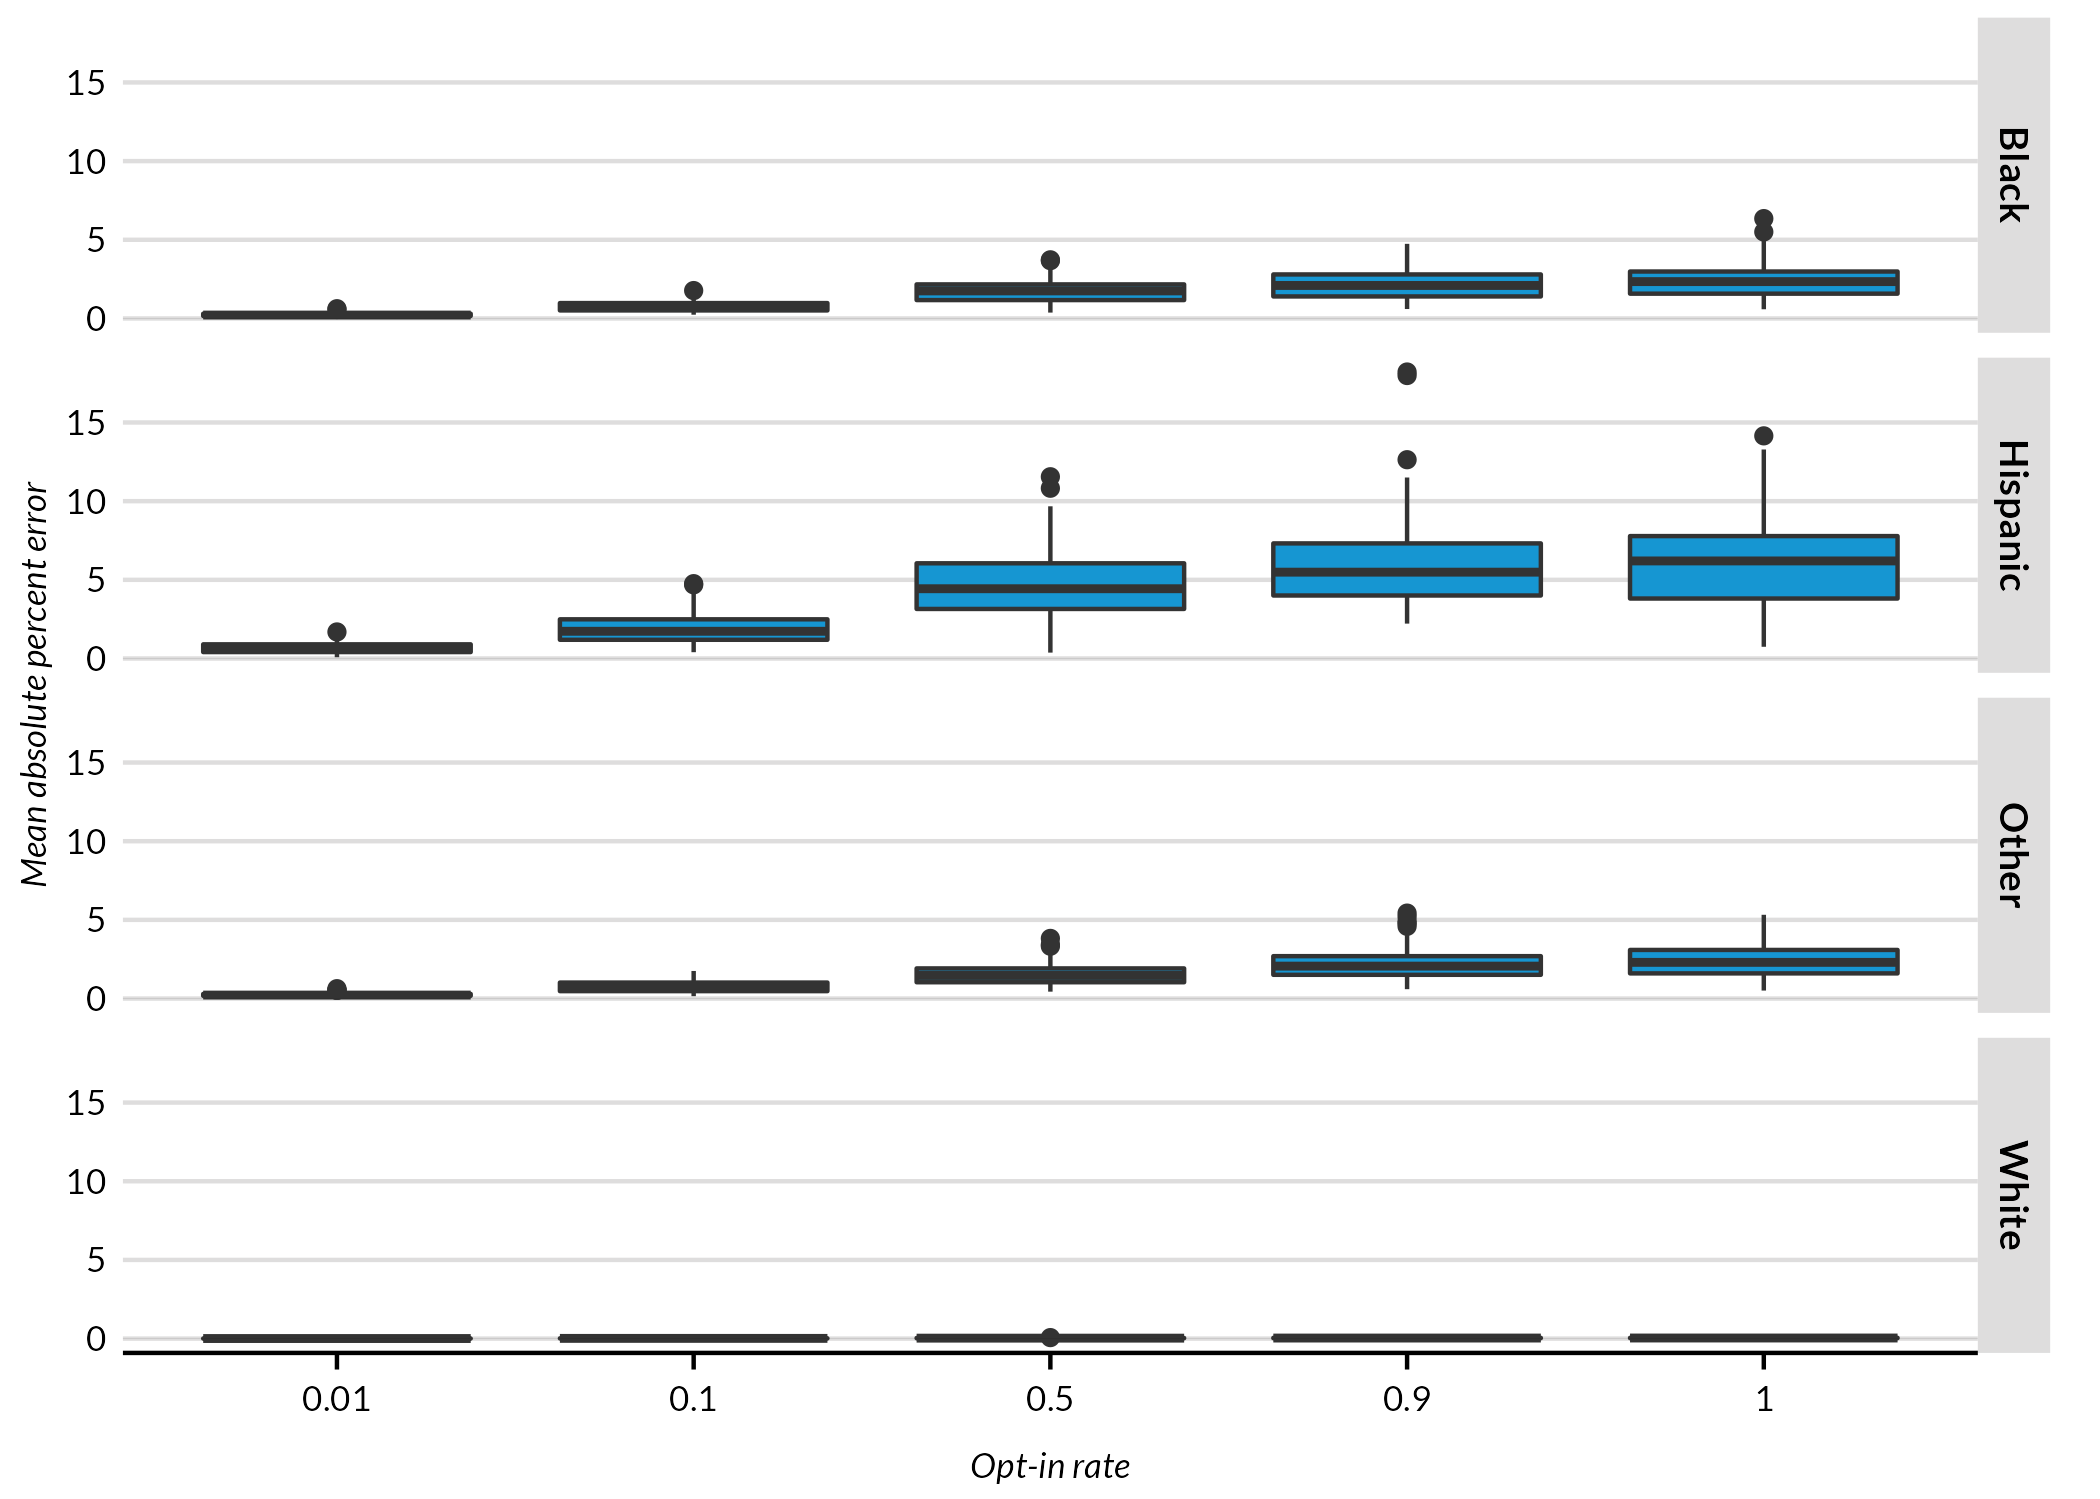
\includegraphics[width=4in]{../figures/groups_ia.png}
    \label{fig:groups_ia}
\end{figure}

According to the 2010 Census Redistricting Data (Public Law 94-171)
Summary File, the population of Washington DC was 38\% white,
non-Hispanic and 51\% Black, non-Hispanic, and the population of Iowa
was 91\% white, non-Hispanic. For both states, mean percent error is
smallest for these relatively large groups, reflecting the larger sample
sizes. Error tends to be relatively larger, and with larger spreads, for
the smaller groups in both places.

The opt-in framework offers a solution path to improve data accuracy for
these smaller racial/ethnic groups. For example, the median absolute
percent error for the Hispanic group is roughly 3.5\% in Washington, DC
and 6\% in Iowa when there is 100\% opt in, or when all respondents are
subjected to disclosure protections. These error values shrink to about
1.5\% and 2\%, respectively, with a group opt-in rate of 10\%. Given the
properties of formal privacy, the privacy protections afforded to those
who opt-in are unaffected by those who choose to forego protections.

With an opt-in disclosure framework, the US Census Bureau and community
groups could engage in outreach efforts, especially to smaller groups,
to help respondents understand the implications of foregoing disclosure
protections, both for their privacy but also for the wide-ranging
impacts of improving their data quality. This type of outreach could
result in better data quality for these groups, with positive downstream
impacts on representation and funding allocations to communities.

All in all, existing local DP methods generate protected data of overall
lower accuracy than data generated by central models. However, this
demonstration shows the potential of local DP to improve data accuracy
for small groups, while still protecting privacy, with an opt-in DP
framework. This use case motivates further development of local DP
methods and opt in experimentation to improve accuracy results.

\section{Demonstration 2: Synthetic Data for the American Community Survey}

The Census Bureau is investigating the creation of a fully synthetic
American Community Survey paired with a validation server\footnote{https://www.ipums.org/changes-to-census-bureau-data-products}.
The Census Bureau intended to create formally private data by 2025 but
later conceded that the science does not exist yet to comprehensively
implement a formally private solution for the ACS\footnote{https://www.census.gov/newsroom/blogs/random-samplings/2022/12/disclosure-avoidance-protections-acs.html}.
Next, the Census Bureau intended to release a non-formally private ACS
in 2024 but their timeline has been delayed because of legitimate
concerns about the impact of synthetic data.\footnote{https://acsdatacommunity.prb.org/discussion-forum/m/2021-acs-conference-files/147/download}

Synthetic data could potentially harm the usefulness of the American
Community Survey. Groups with fewer observations, including smaller
racial and ethnic groups, could see the biggest losses in data quality.
An opt-in disclosure protection methodology paired with synthetic data
could mitigate the harms of data synthesis and give outreach
organizations a tool to improve data quality.

\subsection{Synthetic Data}

Demonstration 1 focused on summary statistics calculated on microdata.
We now pivot to a demonstration where the goal is to produce
high-quality microdata that can be used for a range of valid analyses.
We will pursue this goal with synthetic data generation.

Synthetic data generation is a statistical disclosure control method
that replaces confidential microdata with pseudo microdata that can
maintain the statistical properties of the confidential data while
limiting disclosure risks. United Nations (2022) and Hu and Bowen (2023)
offer thorough introductions to synthetic data. We will briefly
introduce topics central to this demonstration.

There are two main flavors of synthetic data. With partially synthetic
data, some but not all variables are synthesized (Little 1993). With
fully synthetic data, all variables are synthesized (Rubin 1993). Fully
synthetic data generally provides stronger disclosure protection.

Partially synthetic data maintains a one-to-one mapping between
observations in the synthetic data and observations in the GSDS. This
creates identity disclosure risks and increases attribute disclosure
risks. It also means it is possible to calculate disclosure metrics
based on re-identification (J. P. Reiter and Mitra 2009).

Fully synthetic data don't have a one-to-one mapping because every
record is fully generated. This minimizes identity disclosure risks and
attribute disclosure risks, but dramatically reduces approaches for
evaluating disclosure risks. We create a fully synthetic version of the
ACS for this demonstration.

It is possible to create formally private synthetic data in idealized
situations (Bowen and Snoke 2021). Model-based approaches generally
require discretizing categorical variables. Promising approaches
generate 1-, 2-, and 3-way marginals and then use graphical models to
generate synthetic data (McKenna, Sheldon, and Miklau 2019). Other
approaches use GANs but generally don't work well outside of idealized
situations with modest privacy budgets (Tao et al. 2021). Like the
Census Bureau, we abandon formal privacy for this demonstration because
it is currently infeasible for the ACS. This means we no longer have a
provable bound on the worst-case privacy loss.

We use a fully conditional specification (FCS) to generate synthetic
data. FCS uses a sequential approach to model the joint distribution of
the ACS as a sequence of univariate conditional distributions. We use
non-parametric decision trees and regression trees because they are easy
to fit and model relatively complex distributions with ease (J. Reiter
2005). We modify the decision trees and regression trees so that
predictions are samples from the final nodes instead of using the means
and modes of the nodes. This increases the sample variances in the
synthetic data.

We use the tidysynthesis\footnote{``The tidysynthesis R package.''
  Presentation given at rstudio::conf(2022), Washington, DC, July 25 --
  28.} and syntheval R packages to synthesize data and evaluate
synthetic data.

\subsection{Data}

For this demonstration, we use person-level records from the 2021 1-Year
American Community Survey (ACS). The ACS is a roughly 1-in-100 sample of
households in the US and is the premier source of information for small
area estimation. The 2021 ACS Public Use Microdata Sample (PUMS)
contains about 3.25 million individuals and 1.44 million households. We
implement an opt-in disclosure protection demonstration using synthetic
data and the 2021 1-Year American Community Survey. We access all ACS
data through IPUMS (Ruggles et al., n.d.).

We restrict the data in five important ways to minimize computation and
simplify comparisons. First, we restrict our data to observations from
Florida, Michigan, and Pennsylvania. We chose these states because they
are large states with different types of racial and ethnic diversity.
Second, we restrict our data to heads of households ages 18 or older who
are not in group quarters. This limits structurally missing values.
Furthermore, synthesizing relationships within households is a major
technical challenge (Benedetto and Totty 2020). Third, we only
synthesize a subset of variables.

\begin{itemize}
\tightlist
\item
  State (categorical)
\item
  Sex (binary)
\item
  Age (numeric)
\item
  Marital status (categorical)
\item
  Race (categorical)
\item
  Hispanicity (categorical)
\item
  Any health insurance coverage (binary)
\item
  Educational attainment (categorical)
\item
  Employment status (categorical)
\item
  Labor force participation (binary)
\item
  Total family income (numeric)
\item
  Total personal income (numeric)
\item
  Wage and salary income (numeric)
\item
  Welfare income (numeric)
\item
  Income residual (numeric)
\end{itemize}

The income residual is personal income minus wages and salary and
welfare income. The income residual captures all other sources of income
including business income; Social Security income; SSI income; interest,
dividend, and rental income; retirement income; and other income.

Fourth, we ignore weights during synthesis and when calculating metrics.
Synthesis with weights is an open area of research. Fifth and finally,
we randomly partition the data into two halves. The half we apply
disclosure protection to is the gold standard data set (GSDS). The other
half is a holdout data set (HDS) for calculating disclosure metrics.

PUMS include statistical disclosure limitation to protect the
confidentiality of responses. For example, high incomes are topcoded.
When synthesizing data, the Census Bureau has more observations and
unaltered variables that could improve the quality of the synthesis but
also worsen utility metrics because out metrics do not reflect the
current SDC techniques like sampling and topcoding.

\subsection{Simulations}

To evaluate the benefits and costs of opt-in disclosure protection we
implement a simulation study. We vary two key parameters for each
specification. First, we vary the opt-in rate with the values 0.1, 0.5,
0.9, and 1. For example, 90\% of observations are unaltered and 10\% of
observations are synthesized when the opt-in rate is set to 0.1. All
observations are synthesized when the opt-in rate is 1. We call the
result of this SDC approach candidate data. The opt-in decision for each
observation is stochastic. We use a function to set the probability of
opt-in and then randomly select the opt-in decision based on that
probability. Second, we vary the nature of the opt-in. Under the default
settings, all observations have the same opt-in probability within a
specification.

It's plausible that different racial and ethnic groups would opt into
disclosure protections at different rates. We vary individual opt-in
propensities based on race. In addition to equal opt-in probabilities,
we implement a white multiplier such that white individuals opt in at
half the rate of other individuals (0.5) and twice the rate of other
individuals (2). The white multiplier is approximate because the opt-in
decisions are stochastic and because the multiplier is imprecise at high
levels of opt in.

We need to pick an order to synthesize the variables since we adopt a
sequential approach. Typically, more information is preserved for a
synthetic variable by moving it from later in the synthesis order to
earlier in the synthesis order. We prioritize race and ethnicity. Next,
we synthesize the remaining categorical variables. Next, we synthesize
age and educational attainment. We treat both as numeric variables.
Finally, we synthesize all of the income variables.

We implement a simple synthesis without much customization. We use the
rpart implementation of decision trees and regression trees (Therneau
and Atkinson 2022) using their default values (minsplit = 20, minbucket
= 8, and cp = 0.01). These parameters keep the trees from going too deep
and overfitting the data.

We run each specification five times to evaluate the
simulation-to-simulation variation in metrics.

\subsection{Evaluation}

We evaluate the results of the simulations with general utility metrics,
specific utility metrics, and disclosure risk metrics. Descriptions of
each metrics are available in the appendix. Complete results are
available in the Urban Institute data catalog.

General utility measures the univariate and multivariate distributional
similarity between the gold standard data and the candidate data (e.g.,
comparing the medians for all numeric variables). Specific utility
measures the similarity of results for a specific analysis of the gold
standard data and candidate data (e.g., comparing the coefficients in
regression models). Disclosure risk metrics \emph{estimate} the risk of
attribute and membership inference attacks.

We calculate the following metrics for all simulations:

\textbf{General utility}

\begin{itemize}
\tightlist
\item
  Absolute error for proportions for all categorical variables
\item
  Absolute error for proportions for all categorical variables by
  simplified race/ethnicity and detailed race
\item
  Absolute proportion error for means for all numeric variables
\item
  Absolute proportion error for means for all numeric variables by
  simplified race/ethnicity and detailed race
\item
  Proportion error in percentiles for numeric variables
\item
  k-marginal score for all 1-way, 2-way, and 3-way marginals for
  categorical variables
\item
  Mean absolute error in pairwise correlation coefficients for numeric
  variables
\item
  Discriminator ROC AUC
\end{itemize}

\textbf{Specific utility}

\begin{itemize}
\tightlist
\item
  Regression confidence interval overlap for a Mincer model
\end{itemize}

\textbf{Disclosure risk}

\begin{itemize}
\tightlist
\item
  \(\ell\)-diversity for regression trees summarized for each numeric
  variable
\item
  Attribute inference test on welfare income
\item
  Membership inference test
\end{itemize}

\subsection{Results and Discussion}

We have two main concerns with opt-in fully synthetic data. First, the
approach may lead to untenable disclosure risks. Second, the utility
improvements from including unaltered records in released data may be
dampened by synthetic data with worse utility because the synthesizer is
trained on smaller and non-random subsets of the GSDS. Essentially, as
opt-in decreases the number of observations in the training data
decreases, which could lead to terrible models for the synthetic data.

Our demonstration suggests that opt-in fully synthetic data do not
significantly increase disclosure risks. We also observe that all
utility metrics improve with the introduction of an opt-in and improve
as the opt-in rate decreases. Most of the utility metrics are
surprisingly resilient to differential rates of opt-in for white
vs.~non-white respondents. Our results support the idea that opt-in
approaches to synthetic data can improve data quality with minimal
changes to disclosure risks.

\textbf{Multivariate Utility}

\begin{figure}[!htb]
    \caption{Low Opt-In Rates Dramatically Improve Discriminant Metrics}
    \centering
    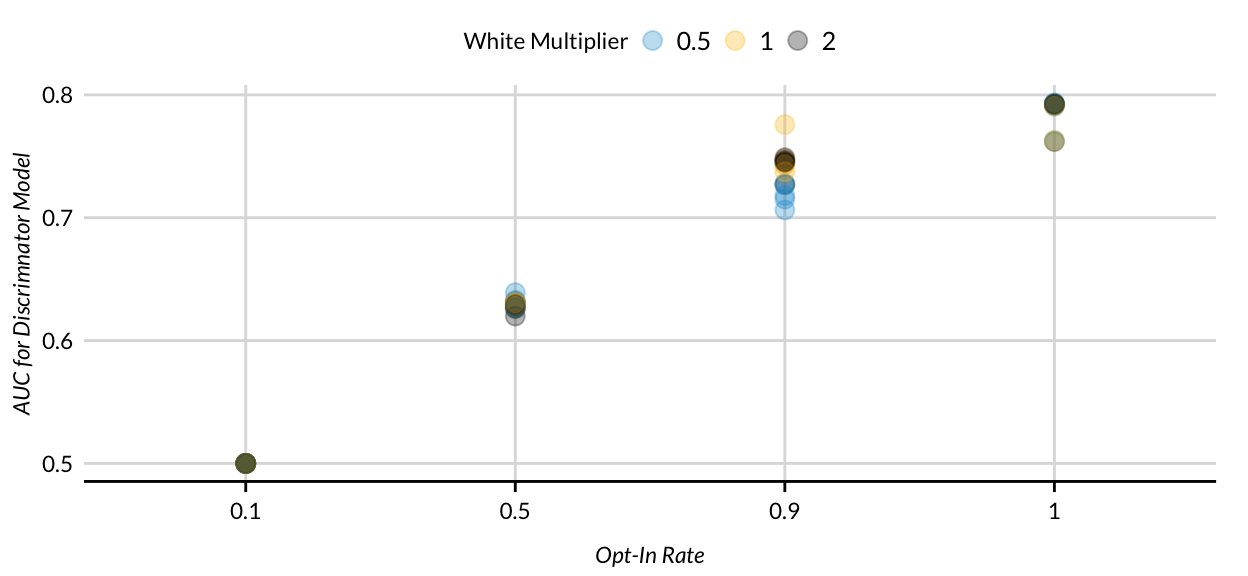
\includegraphics[width=6.5in]{../analysis/figures/discriminator-auc-1.png}
    \label{fig:discriminator}
\end{figure}

We start with multivariate utility. The discriminator AUC, shown in
figure \ref{fig:discriminator}, is high when all observations opt-in to
disclosure protections and quickly declines with lower opt-in rates.
This suggests that a simple predictive model has difficulty
distinguishing between the synthetic data and the GSDS after the
introduction of opt-in synthesis.

\begin{figure}[!htb]
    \caption{Low Opt-In Improves Synthetic Correlations}
    \centering
    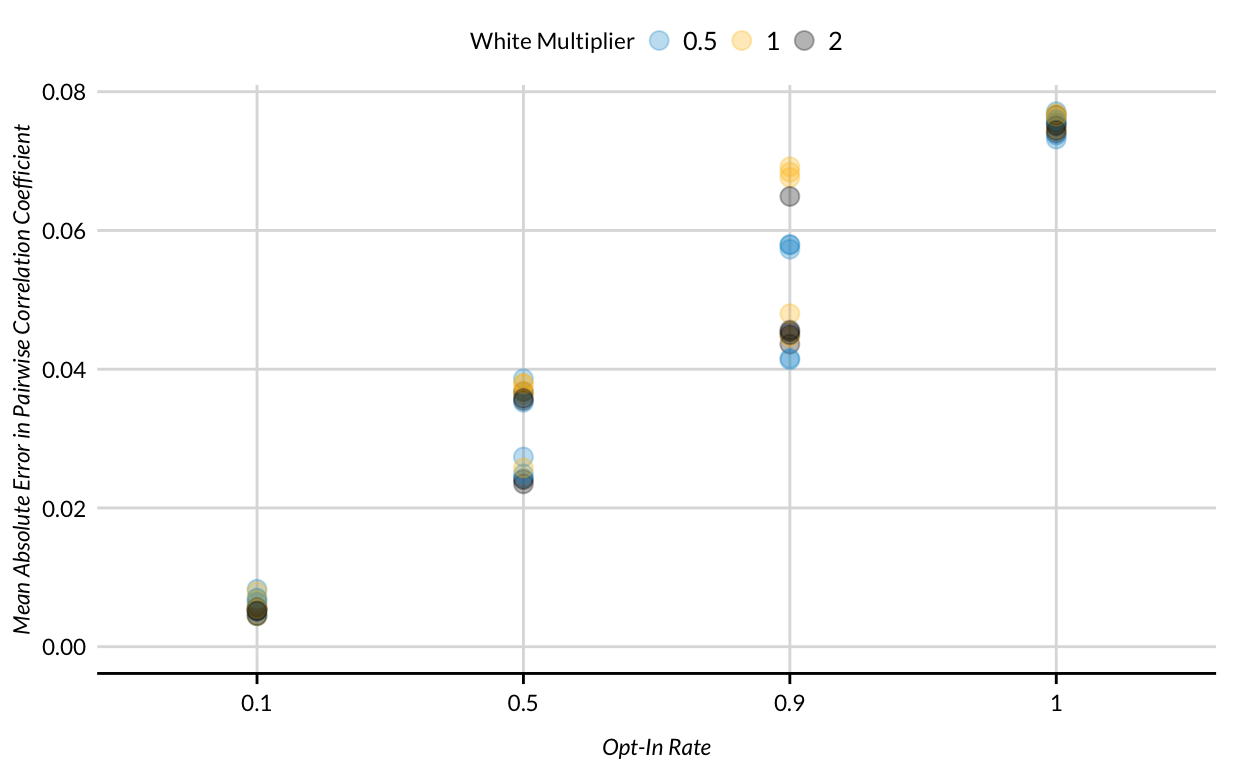
\includegraphics[width=6.5in]{../analysis/figures/correlation-difference-1.png}
    \label{fig:correlation-difference}
\end{figure}

The correlation difference, shown in figure
\ref{fig:correlation-difference} is modest for all opt-in rates and
improves with low levels of opt-in.

Finally, regression estimates dramatically improve with low levels of
opt-in. Figure \ref{fig:regression} shows that the gap between
confidence intervals, which is about six times the length of the
confidence interval with full opt-in disclosure protection, fully
disappears with low levels of opt-in.

\begin{figure}[!htb]
    \caption{Coefficient Estimates are Closer with Low Opt-In Levels}
    \centering
    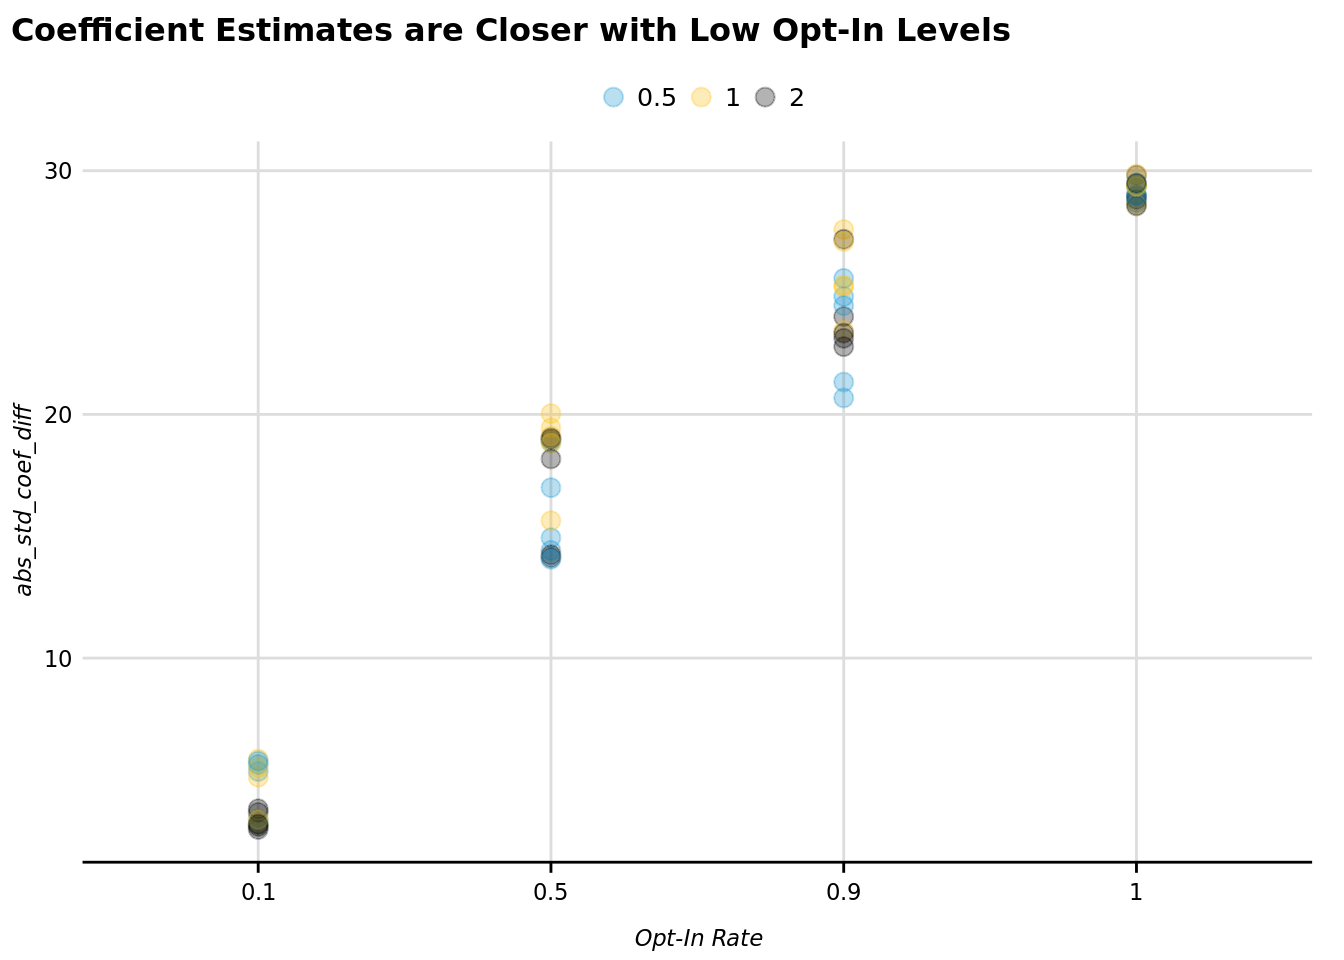
\includegraphics[width=6.5in]{../analysis/figures/regression-overlap-1.png}
    \label{fig:regression}
\end{figure}

\textbf{Univaritate Utility}

We next zoom in on specific variables and subsets of variables. The
categorical utility of the synthetic data is very high for all scenarios
but improves marginally with low opt-in rates.

Figure \ref{fig:proportions} shows the error in proportions for all
categories of all categorical variables. Figure
\ref{fig:proportions-race-ethnicity} shows the proportions for all
classes of all categorical variables disaggregated into four
race/ethnicity groups. Some race/ethnicity groups are poorly represented
in the synthetic data. For example, the Black proportions for ``Married,
spouse present'' and ``Never married, spouse not present'' are very
wrong in the synthetic data because the estimates are attenuated to the
proportions in the majority group. Some of these differences can be
refined by using different hyperparameters during the synthesis process.

\begin{figure}[!htb]
    \caption{Low Opt-In Modestly Improves Univariate Proportion Estimates}
    \centering
    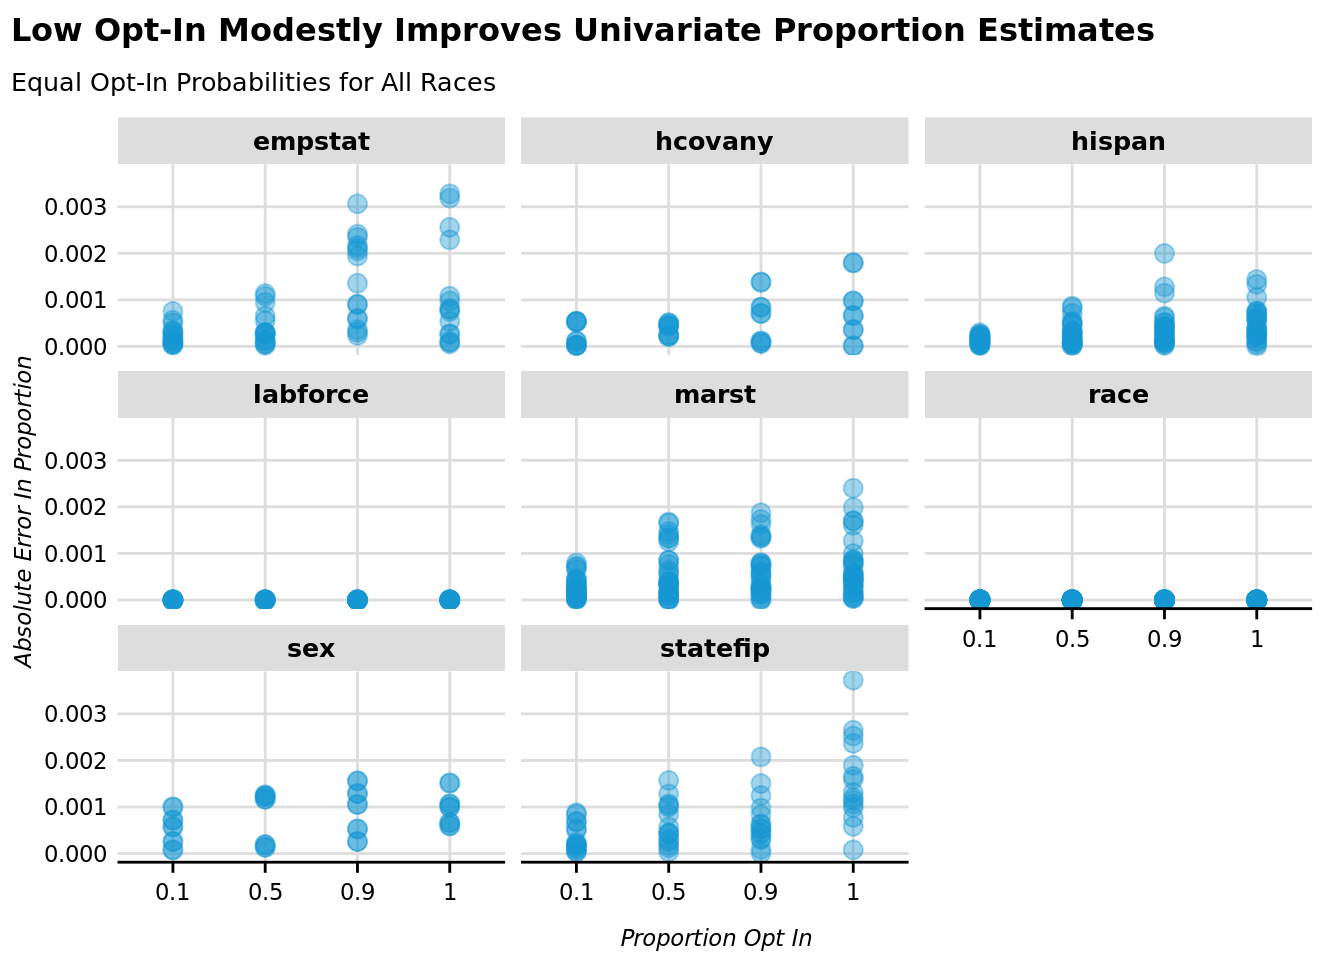
\includegraphics[width=6.5in]{../analysis/figures/proportions-1.png}
    \label{fig:proportions}
\end{figure}

\begin{figure}[!htb]
    \caption{Low Opt-In Reduces Major Racial/Ethnic Errors in Estimates}
    \centering
    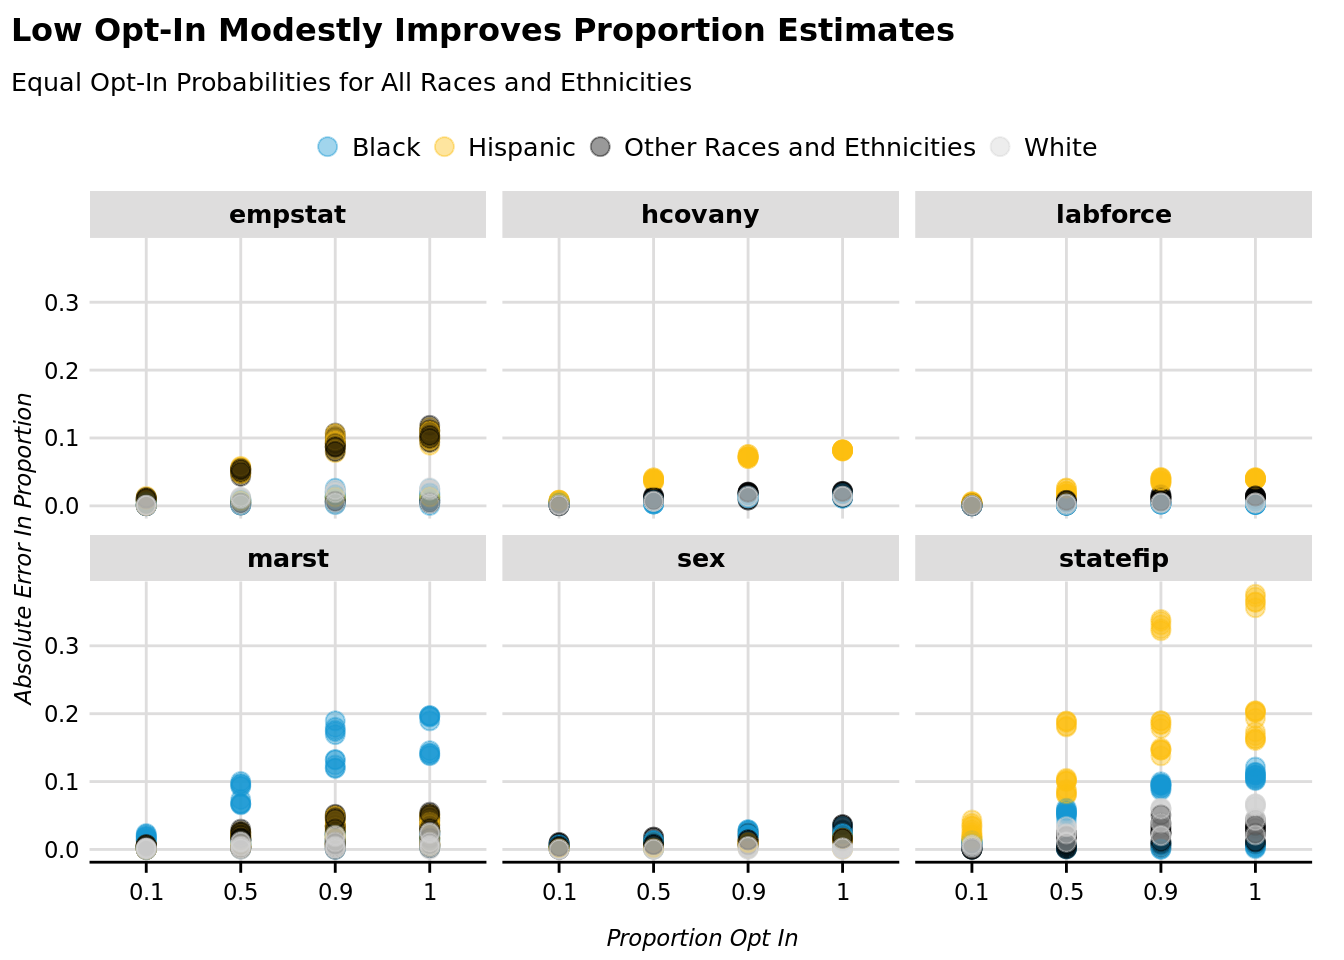
\includegraphics[width=6.5in]{../analysis/figures/proportions-3.png}
    \label{fig:proportions-race-ethnicity}
\end{figure}

We see a similar patterns when reviewing the proportion of indiduals
with Salaries or Wages. Figure \ref{fig:prop-wages} shows that the
synthetic data generally overestimates the number of white people with
salaries and wages and underestimates for Hispanic and Other Races and
Ethnicities.

\begin{figure}[!htb]
    \caption{Low Opt-In Improves Estimates of the Proportions of People with Salaries and Wages}
    \centering
    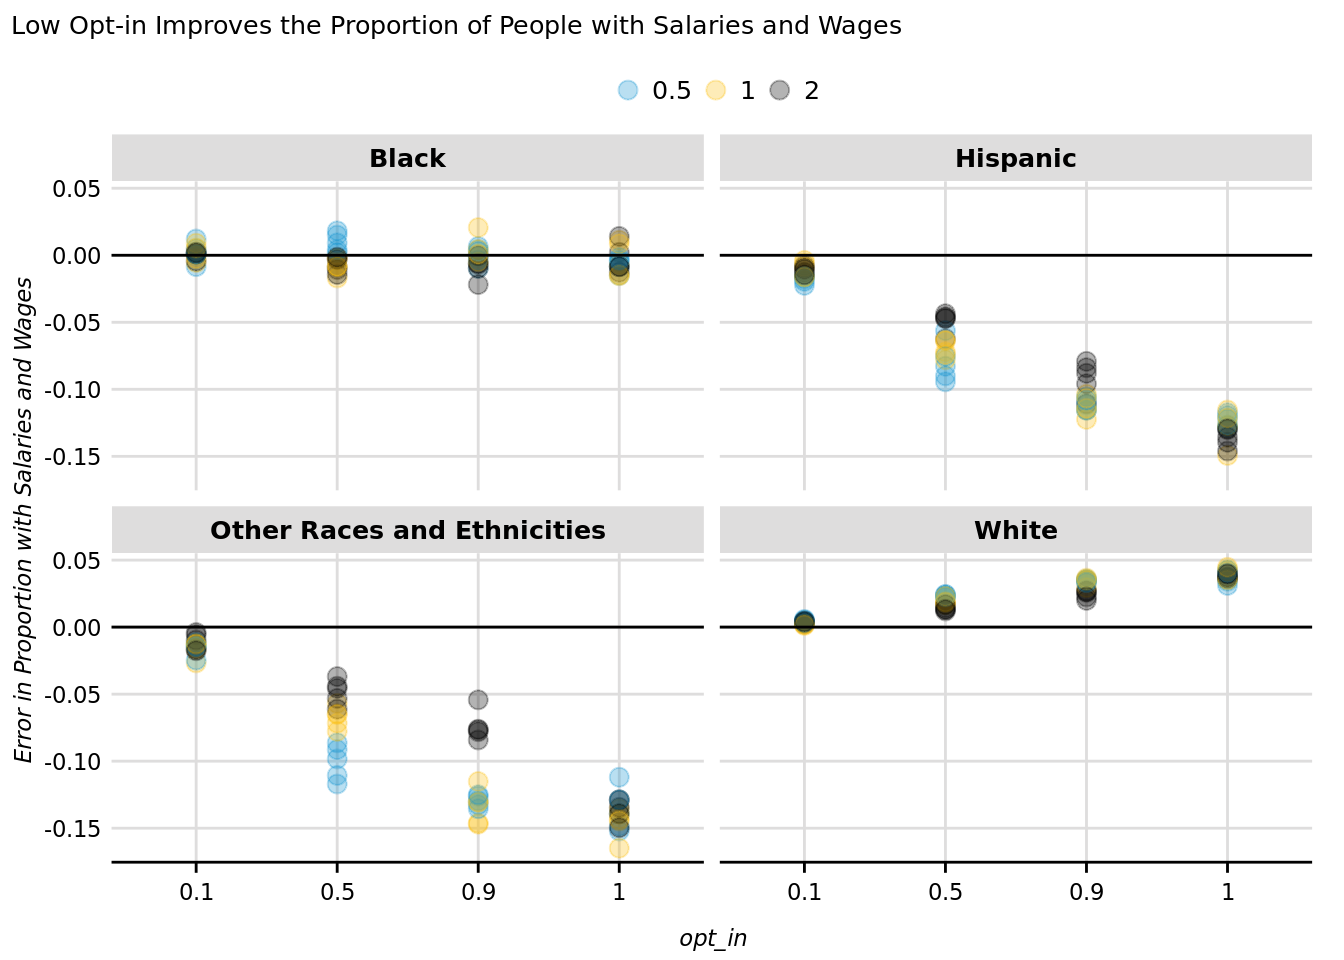
\includegraphics[width=6.5in]{../analysis/figures/proportion-with-wages-3.png}
    \label{fig:prop-wages}
\end{figure}

The 1-marginal score for the synthetic data is always better than the
1-marginal score for the holdout data. The results flip for the
2-marginal score and 3-marginal score. In all three cases, low levels of
opt-in dramatically improve the results. Figure \ref{fig:kmarginals}
shows the k-marginal score for 1-marginals and 3-marginals.

\begin{figure}[!htb]
    \caption{Low Opt-In Improves Higher-Dimensional Distributions}
    \centering
    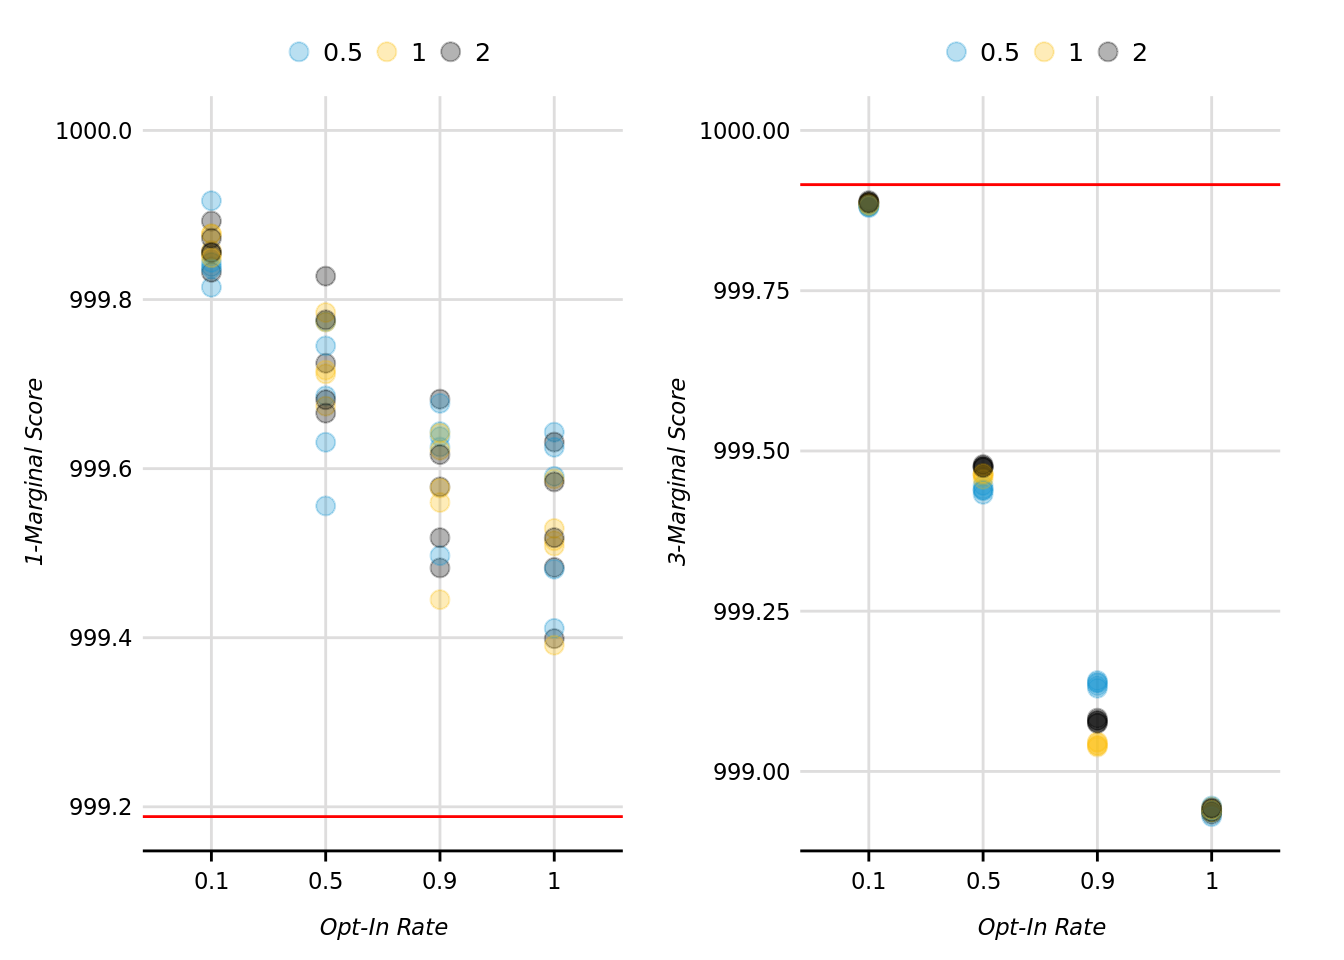
\includegraphics[width=6.5in]{../analysis/figures/kmarginals-4.png}
    \label{fig:kmarginals}
\end{figure}

The syntheses have mixed results for numeric variables. Figure
\ref{fig:family-income} shows that all syntheses closely match the
distribution of total family income. The only major errors are for the
minimum and maximum values.

\begin{figure}[!htb]
    \caption{All Syntheses Recreate the Total Family Income Distribution}
    \centering
    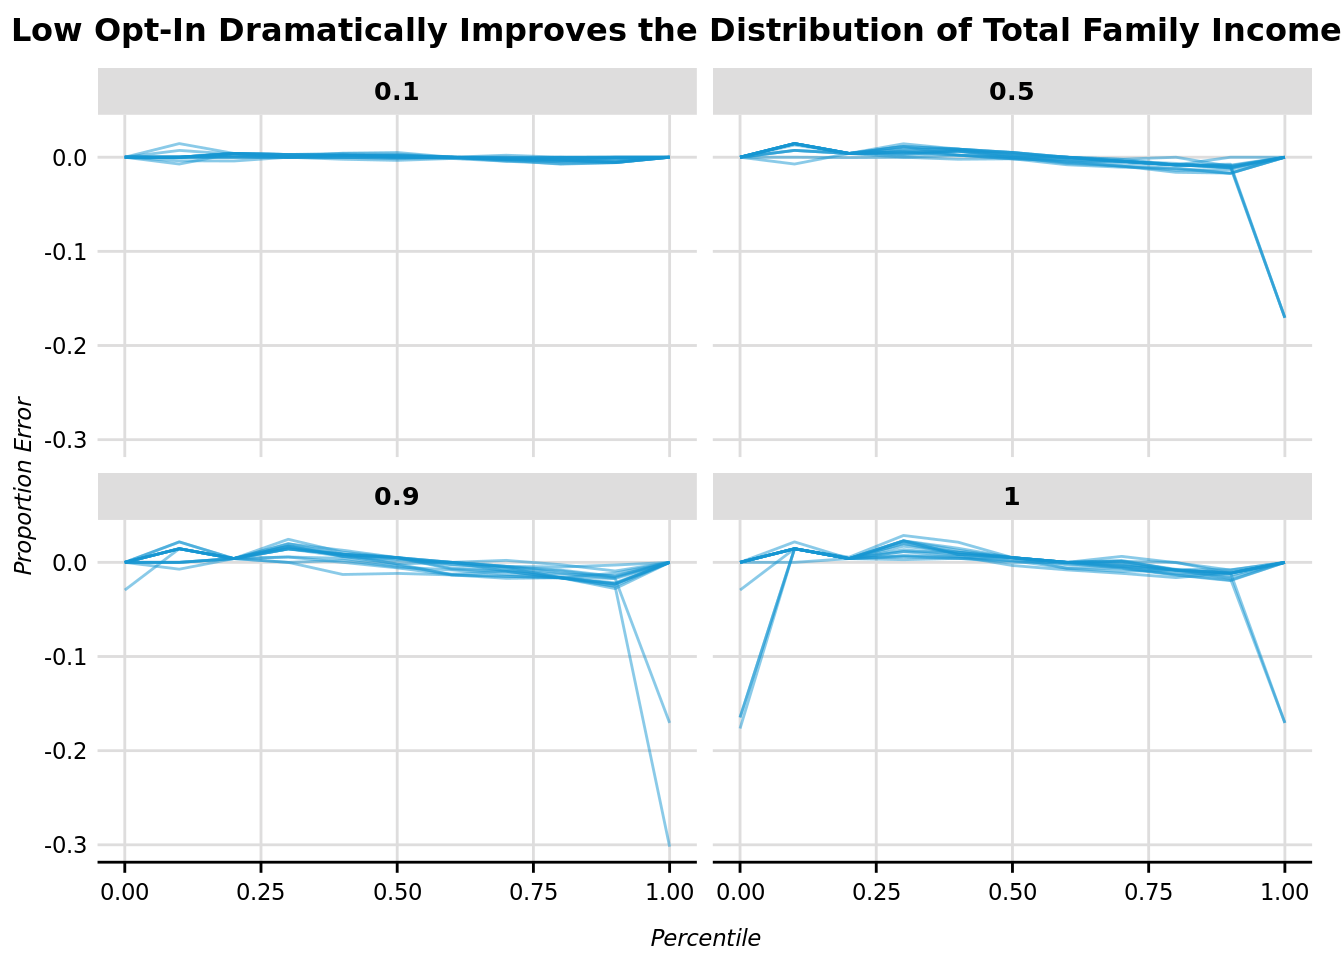
\includegraphics[width=6.5in]{../analysis/figures/percentiles-2.png}
    \label{fig:family-income}
\end{figure}

The syntheses miss the distribution of salary and wage income, shown in
figure \ref{fig:wage-income} but the results improve dramatically with
low levels of opt-in.

\begin{figure}[!htb]
    \caption{Low Opt-In Improves the Distribution of Salary and Wage Income}
    \centering
    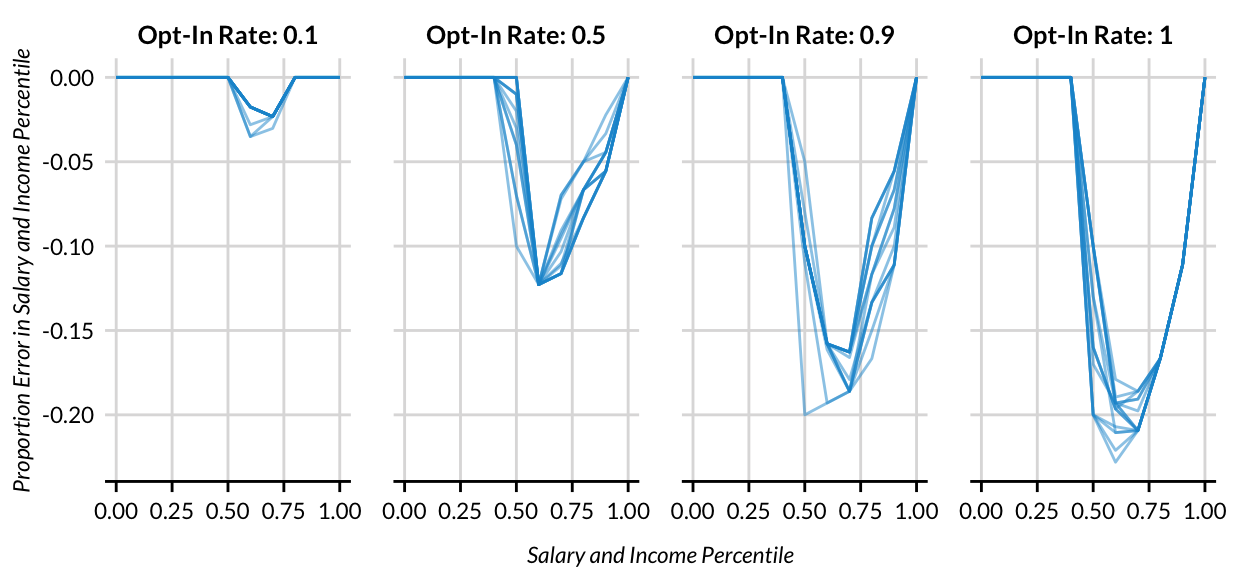
\includegraphics[width=6.5in]{../analysis/figures/percentiles-1.png}
    \label{fig:wage-income}
\end{figure}

\textbf{Disclosure Risks}

The synthesizer demonstrates promising \(\ell\)-diversity for all
syntheses. This is unsurprising since we use conservative
hyperparameters for the decision trees and regression trees. In the
worst-case situation, less than 0.5\% of values for one variable come
from nodes in regression trees with fewer than three unique values.

In Figure \ref{fig:membership}, the AUC for the membership inference
attack is close to 0.5. Given the synthetic data, an attacker would
struggle to tell if a confidential record is from the GSDS or holdout
data using distance-based matching.

\begin{figure}[!htb]
    \caption{No SYnthesis Demonstrates High Membership Inference Risks}
    \centering
    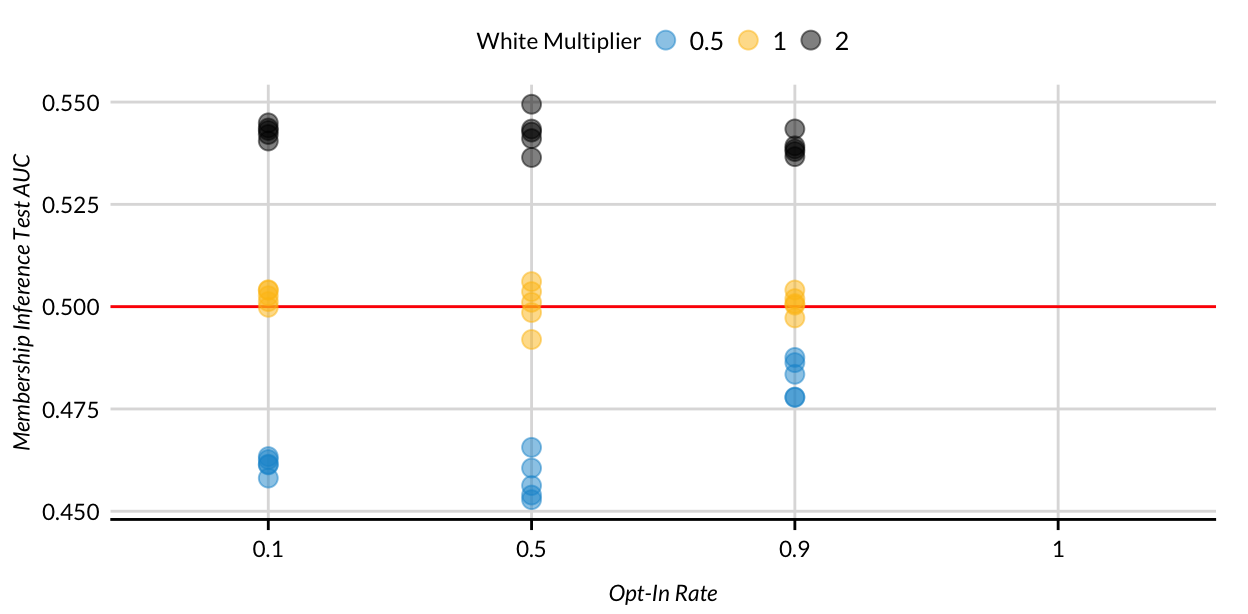
\includegraphics[width=6.5in]{../analysis/figures/membership-inference-1.png}
    \label{fig:membership}
\end{figure}

Finally, the RMSE for the attribute inference test from the synthetic
data is always lower than the RMSE for a model trained on the holdout
data. Using a simple predictive model, this suggests that the synthetic
data are not copying chance features of the GSDS. These disclosure
metrics enable us to infer the disclosive properties of the synthetic
but they don't not provide a bound or guarantee on the disclosure risks
of the synthetic data. This is a major disadvantage of non-formally
private synthetic data when compared with formally private tabulations
like in the first demonstration.

Nonetheless, we believe the results are promising. Allowing individuals
to forego disclosure protections increases data utility without
increasing disclosure risks for the individuals who still want
disclosure protection.

The idea of opt-in disclosure protection with synthetic microdata rests
on one major implementation assumption. We do not label observations
that forego disclosure protections. Doing so could increase disclosure
risks by making differencing attacks easier. Data stewards need to be
careful to not implicitly label the opt-in decision. For example, the
GSDS and observations without opt-in could have precision to the closest
integer when the synthetic records have precision to three decimal
places. In this case, it would be trivial to identify the records with
and without opt-in disclosure protection.

\section{Conclusion}

\hypertarget{ldp}{%
\subsection{LDP}\label{ldp}}

The first demonstration shows the benefits and infeasibility of opt-in
disclosure protections with a differentially private Decennial Census.
The errors introduced when switching from a centralized DP approach to a
local DP approach dramatically outweigh the benefits of embracing opt-in
disclosure protections. Either major methodological breakthroughs for
local DP are needed or opt-in disclosure protections will not improve
the utility-disclosure risk trade off for the Decennial Census.

\hypertarget{synthetic-data}{%
\subsection{Synthetic Data}\label{synthetic-data}}

The second demonstration shows the benefits and feasibility of opt-in
disclosure protections with a fully-synthetic American Community Survey.
In all cases, low levels of opt-in improved the utility of the synthetic
data without worsening disclosure risk metrics. Our synthesis
methodology was simple and suffered from some errors including major
errors for certain race and ethnicity groups. Low levels of opt-in
mitigated many of these issues.

Ample followup work is needed to explore the implementation of opt-in
disclosure protection. We do not address questionnaire design and giving
respondents clear information so they can provide informed consent.
These implementation decisions inform the ethics of opt-in disclosure
protection and would unambiguously affect the opt-in rate. We also only
allow for unit opt-in disclosure protection and do not consider item
opt-in disclosure protection. Item opt-in disclosure protection would be
more difficult to implement but would give respondents even more control
over their data.

The Census Bureau is wrestling with significant outstanding technical
challenges for producing a fully synthetic ACS. Furthermore, the ACS is
protected by Title 13 and would likely need legal changes to allow for
an opt-in approach to disclosure protection.

The Survey of Earned Doctorates (SED) could be an ideal candidate for
evaluating this approach. The survey is a census of persons who recently
earned doctorate degrees. This population would be easier to inform
because of their research backgrounds. The SED has remarkably high
response rates and we speculate that the population would opt-in to
disclosure protections at very low rates. Furthermore, the file avoids
many of the technical challenges currently facing a synthetic ACS.

\subsection{Metrics Appendix}

% Footer Formatting: DO NOT CHANGE -----------------------------------
\fancyfoot{}

\fancyfoot[LE]{\colorbox{urban-footergray}{\makebox(0.2, 0.12)[r]{\fontsize{7.5}{0}\selectfont\bfseries{\MakeUppercase{}\hspace{0.2in}}}}\colorbox{urban-gold}{\makebox(0.2, 0.12)[c]{\fontsize{7.5}{0}\selectfont\bfseries{\MakeUppercase\thepage}}}\colorbox{urban-footergray}{\makebox(5.64, 0.12)[r]{\fontsize{7.5}{0}\selectfont\bfseries{\MakeUppercase{Appendix}\hspace{0.2in}}}}}

\fancyfoot[RO]{\colorbox{urban-footergray}{\makebox(5.64, 0.12)[l]{\fontsize{7.5}{0}\selectfont\bfseries{\hspace{0.2in}\MakeUppercase{Appendix}}}}\colorbox{urban-gold}{\makebox(0.2, 0.12)[c]{\fontsize{7.5}{0}\selectfont\bfseries{\MakeUppercase\thepage}}}\colorbox{urban-footergray}{\makebox(0.2, 0.12)[r]{\fontsize{7.5}{0}\selectfont\bfseries{\MakeUppercase{}\hspace{0.2in}}}}}
% Footer Formatting: DO NOT CHANGE -----------------------------------
%%%%%%%%%%%%%%%%%%%%%%%%%%%%%%%%%%%% Appendix %%%%%%%%%%%%%%%%%%%%%%%%%%%%%%%%%%%%%%%%%%%
\begin{FlushLeft}
    \part{Appendix Letter. Appendix Title in Title Case}
\end{FlushLeft}

Use the same text styles you used in the main report.

% Footer Formatting: DO NOT CHANGE -----------------------------------
\fancyfoot{}

\fancyfoot[LE]{\colorbox{urban-footergray}{\makebox(0.2, 0.12)[r]{\fontsize{7.5}{0}\selectfont\bfseries{\MakeUppercase{}\hspace{0.2in}}}}\colorbox{urban-gold}{\makebox(0.2, 0.12)[c]{\fontsize{7.5}{0}\selectfont\bfseries{\MakeUppercase\thepage}}}\colorbox{urban-footergray}{\makebox(5.64, 0.12)[r]{\fontsize{7.5}{0}\selectfont\bfseries{\MakeUppercase{Notes}\hspace{0.2in}}}}}

\fancyfoot[RO]{\colorbox{urban-footergray}{\makebox(5.64, 0.12)[l]{\fontsize{7.5}{0}\selectfont\bfseries{\hspace{0.2in}\MakeUppercase{Notes}}}}\colorbox{urban-gold}{\makebox(0.2, 0.12)[c]{\fontsize{7.5}{0}\selectfont\bfseries{\MakeUppercase\thepage}}}\colorbox{urban-footergray}{\makebox(0.2, 0.12)[r]{\fontsize{7.5}{0}\selectfont\bfseries{\MakeUppercase{}\hspace{0.2in}}}}}

% Notes Title Formatting
\renewcommand\notesname{\color{urban-blue}\fontsize{28}{0pt}\selectfont Notes\vspace{-12pt}}
% Footer Formatting: DO NOT CHANGE -----------------------------------

%%%%%%%%%%%%%%%%%%%%%%%%%%%%%%%%%%%% Notes %%%%%%%%%%%%%%%%%%%%%%%%%%%%%%%%%%%%%%%%%%%%%%
\addcontentsline{toc}{part}{Notes}
\theendnotes

% Footer Formatting: DO NOT CHANGE -----------------------------------
\fancyfoot{}

\fancyfoot[LE]{\colorbox{urban-footergray}{\makebox(0.2, 0.12)[r]{\fontsize{7.5}{0}\selectfont\bfseries{\MakeUppercase{}\hspace{0.2in}}}}\colorbox{urban-gold}{\makebox(0.2, 0.12)[c]{\fontsize{7.5}{0}\selectfont\bfseries{\MakeUppercase\thepage}}}\colorbox{urban-footergray}{\makebox(5.64, 0.12)[r]{\fontsize{7.5}{0}\selectfont\bfseries{\MakeUppercase{References}\hspace{0.2in}}}}}

\fancyfoot[RO]{\colorbox{urban-footergray}{\makebox(5.64, 0.12)[l]{\fontsize{7.5}{0}\selectfont\bfseries{\hspace{0.2in}\MakeUppercase{References}}}}\colorbox{urban-gold}{\makebox(0.2, 0.12)[c]{\fontsize{7.5}{0}\selectfont\bfseries{\MakeUppercase\thepage}}}\colorbox{urban-footergray}{\makebox(0.2, 0.12)[r]{\fontsize{7.5}{0}\selectfont\bfseries{\MakeUppercase{}\hspace{0.2in}}}}}
% Footer Formatting: DO NOT CHANGE -----------------------------------
%%%%%%%%%%%%%%%%%%%%%%%%%%%%%%%%%%%% References %%%%%%%%%%%%%%%%%%%%%%%%%%%%%%%%%%%%%%%%%
\addcontentsline{toc}{part}{References}

\printbibliography[title={\color{urban-blue}\fontsize{28}{18}\selectfont References}]

% Footer Formatting: DO NOT CHANGE -----------------------------------
\fancyfoot{}

\fancyfoot[LE]{\colorbox{urban-footergray}{\makebox(0.2, 0.12)[r]{\fontsize{7.5}{0}\selectfont\bfseries{\MakeUppercase{}\hspace{0.2in}}}}\colorbox{urban-gold}{\makebox(0.2, 0.12)[c]{\fontsize{7.5}{0}\selectfont\bfseries{\MakeUppercase\thepage}}}\colorbox{urban-footergray}{\makebox(5.64, 0.12)[r]{\fontsize{7.5}{0}\selectfont\bfseries{\MakeUppercase{About the Authors}\hspace{0.2in}}}}}

\fancyfoot[RO]{\colorbox{urban-footergray}{\makebox(5.64, 0.12)[l]{\fontsize{7.5}{0}\selectfont\bfseries{\hspace{0.2in}\MakeUppercase{About the Authors}}}}\colorbox{urban-gold}{\makebox(0.2, 0.12)[c]{\fontsize{7.5}{0}\selectfont\bfseries{\MakeUppercase\thepage}}}\colorbox{urban-footergray}{\makebox(0.2, 0.12)[r]{\fontsize{7.5}{0}\selectfont\bfseries{\MakeUppercase{}\hspace{0.2in}}}}}
% Footer Formatting: DO NOT CHANGE -----------------------------------
%%%%%%%%%%%%%%%%%%%%%%%%%%%%%%%%%%%% About Author %%%%%%%%%%%%%%%%%%%%%%%%%%%%%%%%%%%%%%
\part{About the Authors}

\textbf{Aaron R. Williams} but the rest of the text lightface. Use Author Bios--First style for the introductory paragraph of each bio. You can paste your bio from your author page on the Urban website (and condense it if needed) here.\\
If your bio is more than one paragraph long, use Author Bios--Additional for any subsequent paragraphs. This style suppresses spacing between paragraphs.\\
Author bios no longer include photos.

\noindent\textbf{Jennifer Andre} but the rest of the text lightface. Use Author Bios--First style for the introductory paragraph of each bio. You can paste your bio from your author page on the Urban website (and condense it if needed) here.\\
If your bio is more than one paragraph long, use Author Bios--Additional for any subsequent paragraphs. This style suppresses spacing between paragraphs.\\
Author bios no longer include photos.

%%%%%%%%%%%%%%%%%%%%%%%%%%%%%%%%%%%% Statement of Independence %%%%%%%%%%%%%%%%%%%%%%%%%%
\addcontentsline{toc}{part}{Statement of Independence}
\thispagestyle{empty} 

\about{S\scalebox{0.8}{tatement of} I\scalebox{0.8}{ndependence}}
\vspace{-5pt}
\boilerplate{The Urban Institute strives to meet the highest standards of integrity and quality in its research and analyses and in the evidence-based policy recommendations offered by its researchers and experts. We believe that operating consistent with the values of independence, rigor, and transparency is essential to maintaining those standards. As an organization, the Urban Institute does not take positions on issues, but it does empower and support its experts in sharing their own evidence-based views and policy recommendations that have been shaped by scholarship. Funders do not determine our research findings or the insights and recommendations of our experts. Urban scholars and experts are expected to be objective and follow the evidence wherever it may lead.}

\newpage
\thispagestyle{empty}

\begin{textblock*}{8.5in}[1, 1](8.5in, 11in)
    \noindent
\includegraphics[width=\paperwidth,height=\paperheight]{images/back.pdf}
\end{textblock*}

\hypertarget{refs}{}
\begin{CSLReferences}{1}{0}
\leavevmode\vadjust pre{\hypertarget{ref-abowd2018}{}}%
Abowd, John M. 2018. {``Protecting the Confidentiality of Americas
Statistics: Adopting Modern Disclosure Avoidance Methods at the Census
Bureau.''}
\url{https://www.census.gov/newsroom/blogs/research-matters/2018/08/protecting_the_confi.html}.

\leavevmode\vadjust pre{\hypertarget{ref-abowd2022a}{}}%
Abowd, John, Robert Ashmead, Ryan Cumings-Menon, Simson Garfinkel, Micah
Heineck, Christine Heiss, Robert Johns, et al. 2022. {``The 2020 Census
Disclosure Avoidance System TopDown Algorithm.''} \emph{Harvard Data
Science Review}, no. Special Issue 2 (June).
\url{https://doi.org/10.1162/99608f92.529e3cb9}.

\leavevmode\vadjust pre{\hypertarget{ref-axelrod2022}{}}%
Axelrod, Judah, Karolina Ramos, and Rebecca Bullied. 2022.
{``Opportunities and Challenges in Using Private-Sector Data for Racial
Equity Analysis.''}

\leavevmode\vadjust pre{\hypertarget{ref-benedetto2020}{}}%
Benedetto, Gary, and Evan Totty. 2020. {``Synthesizing Familial Linkages
for Privacy in Microdata.''} CED-DA Working Paper.

\leavevmode\vadjust pre{\hypertarget{ref-bowen2021}{}}%
Bowen, Claire McKay, and Joshua Snoke. 2021. {``Comparative Study of
Differentially Private Synthetic Data Algorithms from the NIST PSCR
Differential Privacy Synthetic Data Challenge.''} \emph{Journal of
Privacy and Confidentiality} 11 (1).
\url{https://doi.org/10.29012/jpc.748}.

\leavevmode\vadjust pre{\hypertarget{ref-bowen2022}{}}%
Bowen, Claire McKay, Aaron R Williams, and Madeline Pickens. 2022.
{``Decennial Disclosure: An Explainer on Formal Privacy and the TopDown
Algorithm.''}

\leavevmode\vadjust pre{\hypertarget{ref-daily2022a}{}}%
Daily, Donna. 2022. {``Disclosure Avoidance Protections for the American
Community Survey.''}
\url{https://www.census.gov/newsroom/blogs/random-samplings/2022/12/disclosure-avoidance-protections-acs.html}.

\leavevmode\vadjust pre{\hypertarget{ref-dwork2006c}{}}%
Dwork, Cynthia, Frank McSherry, Kobbi Nissim, and Adam Smith. 2006.
{``Calibrating Noise to Sensitivity in Private Data Analysis.''} In,
edited by Shai Halevi and Tal Rabin, 3876:265--84. Berlin, Heidelberg:
Springer Berlin Heidelberg.
\url{http://link.springer.com/10.1007/11681878_14}.

\leavevmode\vadjust pre{\hypertarget{ref-hotchkiss2017a}{}}%
Hotchkiss, Marisa, and Jessica Phelan. 2017. {``Uses of Census Bureau
Data in Federal Funds Distribution: A New Design for the 21st
Century,''} September.
\url{https://www2.census.gov/programs-surveys/decennial/2020/program-management/working-papers/Uses-of-Census-Bureau-Data-in-Federal-Funds-Distribution.pdf}.

\leavevmode\vadjust pre{\hypertarget{ref-hotz2022a}{}}%
Hotz, V. Joseph, and Joseph Salvo. 2022. {``A Chronicle of the
Application of Differential Privacy to the 2020 Census.''} \emph{Harvard
Data Science Review}, June.
\url{https://doi.org/10.1162/99608f92.ff891fe5}.

\leavevmode\vadjust pre{\hypertarget{ref-hu2023}{}}%
Hu, Jingchen, and Claire McKay Bowen. 2023. {``Advancing Microdata
Privacy Protection: A Review of Synthetic Data.''}
\url{https://doi.org/10.48550/ARXIV.2308.00872}.

\leavevmode\vadjust pre{\hypertarget{ref-little1993}{}}%
Little, Roderick JA. 1993. {``Statistical Analysis of Masked Data.''}
\emph{Journal of Official Statistics} 9 (2): 407.
\url{https://www.scb.se/contentassets/ca21efb41fee47d293bbee5bf7be7fb3/statistical-analysis-of-masked-data.pdf}.

\leavevmode\vadjust pre{\hypertarget{ref-mather2019a}{}}%
Mather, Mark, and Paola Scommegna. 2019. {``Why Is the u.s. Census so
Important?''} March.
\url{https://www.prb.org/resources/importance-of-u-s-census/}.

\leavevmode\vadjust pre{\hypertarget{ref-mckenna2019}{}}%
McKenna, Ryan, Daniel Sheldon, and Gerome Miklau. 2019.
{``Graphical-Model Based Estimation and Inference for Differential
Privacy.''} \emph{Proceedings of the 36th International Conference on
Machine Learning} 97: 4435--44.
\url{http://proceedings.mlr.press/v97/mckenna19a/mckenna19a.pdf}.

\leavevmode\vadjust pre{\hypertarget{ref-near2022}{}}%
Near, Joseph P, and Chiké Abuah. 2022. \emph{Programming Differential
Privacy}.

\leavevmode\vadjust pre{\hypertarget{ref-reiter2009}{}}%
Reiter, Jerome P., and Robin Mitra. 2009. {``Estimating Risks of
Identification Disclosure in Partially Synthetic Data.''} \emph{Journal
of Privacy and Confidentiality} 1 (1).
\url{https://doi.org/10.29012/jpc.v1i1.567}.

\leavevmode\vadjust pre{\hypertarget{ref-reiter2005}{}}%
Reiter, JP. 2005. {``Using CART to Generate Partially Synthetic Public
Use Microdata.''} \emph{Journal of Official Statistics} 21 (3): 441.
\url{https://www.proquest.com/docview/1266792149/abstract/B4CAD6D1A888424FPQ/1?accountid=11091}.

\leavevmode\vadjust pre{\hypertarget{ref-rubin1993}{}}%
Rubin, Donald B. 1993. {``Statistical Disclosure Limitation.''}
\emph{Journal of Official Statistics} 9 (2): 461--68.

\leavevmode\vadjust pre{\hypertarget{ref-ruggles}{}}%
Ruggles, Steven, Sarah Flood, Matthew Sobek, Danika Brockman, Grace
Cooper, Stephanie Richards, and Megan Schouwiler. n.d. {``IPUMS USA:
Version 13.0.''} \url{https://doi.org/10.18128/D010.V13.0}.

\leavevmode\vadjust pre{\hypertarget{ref-tao2021}{}}%
Tao, Yuchao, Ryan McKenna, Michael Hay, Ashwin Machanavajjhala, and
Gerome Miklau. 2021. {``Benchmarking Differentially Private Synthetic
Data Generation Algorithms.''}
\url{https://doi.org/10.48550/ARXIV.2112.09238}.

\leavevmode\vadjust pre{\hypertarget{ref-therneau2022}{}}%
Therneau, Terry M., and Elizabeth J. Atkinson. 2022. {``An Introduction
to Recursive Partitioning Using the RPART Routines.''}
\url{https://cran.r-project.org/web/packages/rpart/vignettes/longintro.pdf}.

\leavevmode\vadjust pre{\hypertarget{ref-syntheti2022}{}}%
United Nations, ed. 2022. \emph{Synthetic Data for Official Statistics:
A Starter Guide}. Geneva: United Nations.

\leavevmode\vadjust pre{\hypertarget{ref-unitedstatescensusbureau2017}{}}%
United States Census Bureau. 2017. {``American Community Survey
Information Guide,''} October.

\leavevmode\vadjust pre{\hypertarget{ref-wang2020a}{}}%
Wang, Teng, Xuefeng Zhang, Jingyu Feng, and Xinyu Yang. 2020. {``A
Comprehensive Survey on Local Differential Privacy Toward Data
Statistics and Analysis.''} \emph{Sensors} 20 (24): 7030.
\url{https://doi.org/10.3390/s20247030}.

\leavevmode\vadjust pre{\hypertarget{ref-warner1965a}{}}%
Warner, Stanley L. 1965. {``Randomized Response: A Survey Technique for
Eliminating Evasive Answer Bias.''} \emph{Journal of the American
Statistical Association} 60 (309): 63--69.
\url{https://doi.org/10.1080/01621459.1965.10480775}.

\leavevmode\vadjust pre{\hypertarget{ref-williams2023a}{}}%
Williams, Aaron R., and Claire McKay Bowen. 2023. {``The Promise and
Limitations of Formal Privacy.''} \emph{WIREs Computational Statistics},
May, e1615. \url{https://doi.org/10.1002/wics.1615}.

\end{CSLReferences}



\newpage
\thispagestyle{empty}

\begin{textblock*}{8.5in}[1, 1](8.5in, 11in)
    \noindent
\includegraphics[width=\paperwidth,height=\paperheight]{images/back.pdf}
\end{textblock*}

\end{document}

\end{document}
